\documentclass[11pt,a4paper]{report}
\usepackage[english]{babel}

% math stuff, symbols --------------------------------------
\usepackage{mathrsfs} % fancy math letters
\usepackage{amsmath}
\usepackage{amsfonts}
\usepackage{amssymb}
\usepackage{amsthm}
\usepackage{mathdesign}
\usepackage{slashed}
\usepackage{mathtools}% \usepackage{empheq} is included in mathtools
%------------------------------------------------------------
\usepackage{graphicx}
\usepackage[usenames,dvipsnames,svgnames,table]{xcolor} % more shades than color
\usepackage{fancyhdr}

% caption --------------------------------------------------
\usepackage[font={sl,footnotesize},format=hang,labelfont={bf,sl,small},width=0.8\textwidth]{caption}
\usepackage{subcaption}


% itemize/description/enumerate ----------------------------
\usepackage{enumitem} %pro­vides user con­trol over the lay­out of the three ba­sic list en­vi­ron­ments

% Miscellanea ----------------------------------------------
\usepackage{cite}
\usepackage{calc}
%% LaTeX can manipulate numbers.The calc package provides the common infix notation.
\usepackage{lscape} 
% Set a page in landscape with	\begin{landscape}
\usepackage{centernot}
% prints the sym­bol \not on the fol­low­ing ar­gu­ment. 
% Un­like the de­fault \not com­mand, the sym­bol is hor­i­zon­tally cen­tered. 
\usepackage{mhchem} % Chemistry formulas, Isotopes, etc. 
% see usage here: https://docs.moodle.org/27/en/Chemistry_notation_using_mhchem
\usepackage{listings}%To insert programming code within the document. 
\lstset{breaklines=true}
% Many languages are supported and the output can be customized.

\usepackage[     %pdftex%, 
                 %plainpages = false, %pdfpagelabels, 
                 %pdfpagelayout = useoutlines,
                 bookmarks,
                 bookmarksopen = true,
                 bookmarksnumbered = true,
                 breaklinks = true,
                 linktocpage,
                 %pagebackref,
                 colorlinks = true,  % was true
                 linkcolor = blue,
                 urlcolor  = black,
                 citecolor = blue,
                 anchorcolor = black,
                 hyperindex = true,
                 %hyperfigures
                 ]{hyperref} % manage links within the document or to any URL when you compile in PDF
                 


\usepackage{lineno} %% line numbers 
\usepackage{siunitx} %% Metric international system units


\definecolor{mygreen}{rgb}{0,0.6,0}
\definecolor{mygray}{rgb}{0.5,0.5,0.5}
\definecolor{mymauve}{rgb}{0.58,0,0.82}

\def\name{Gabriele Inghirami and Valentina Rolando}

\lstset{ %
  backgroundcolor=\color{white},   % choose the background color; you must add \usepackage{color} or \usepackage{xcolor}
  basicstyle=\footnotesize,        % the size of the fonts that are used for the code
  breakatwhitespace=false,         % sets if automatic breaks should only happen at whitespace
  breaklines=true,                 % sets automatic line breaking
  captionpos=b,                    % sets the caption-position to bottom
  commentstyle=\color{mygreen},    % comment style
%   deletekeywords={number},            % if you want to delete keywords from the given language
  escapeinside={\%*}{*)},          % if you want to add LaTeX within your code
  extendedchars=true,              % lets you use non-ASCII characters; for 8-bits encodings only, does not work with UTF-8
  frame=single,                    % adds a frame around the code
  keepspaces=true,                 % keeps spaces in text, useful for keeping indentation of code (possibly needs columns=flexible)
  keywordstyle=\color{blue},       % keyword style
  language=fortran,                 % the language of the code
%   morekeywords={*,...},            % if you want to add more keywords to the set
  numbers=left,                    % where to put the line-numbers; possible values are (none, left, right)
  numbersep=5pt,                   % how far the line-numbers are from the code
  numberstyle=\tiny\color{mygray}, % the style that is used for the line-numbers
  rulecolor=\color{black},         % if not set, the frame-color may be changed on line-breaks within not-black text (e.g. comments (green here))
  showspaces=false,                % show spaces everywhere adding particular underscores; it overrides 'showstringspaces'
  showstringspaces=false,          % underline spaces within strings only
  showtabs=false,                  % show tabs within strings adding particular underscores
  stepnumber=2,                    % the step between two line-numbers. If it's 1, each line will be numbered
  stringstyle=\color{mymauve},     % string literal style
  tabsize=2,                       % sets default tabsize to 2 spaces
  title=\lstname                   % show the filename of files included with \lstinputlisting; also try caption instead of title
}



\lstdefinestyle{customtxt}{
  belowcaptionskip=1\baselineskip,
  breaklines=true,
  frame=L,
  xleftmargin=\parindent,
%   language=none,
  showstringspaces=false,
  basicstyle=\footnotesize\ttfamily,
%   keywordstyle=\bfseries\color{green!40!black},
%   commentstyle=\itshape\color{purple!40!black},
%   identifierstyle=\color{blue},
%   stringstyle=\color{orange},
  keywordstyle=\color{black},
  commentstyle=\color{black},
  identifierstyle=\color{black},
  stringstyle=\color{black},
}
\newcommand{\Cred}{\color{red}}
\newcommand{\Cblue}{\color{blue}}
\newcommand*\mygraybox[1]{\colorbox{lightgray}{#1}}
\newcommand{\fo}{Freeze-Out }
\newcommand{\de}{\mathrm{d}}
\newcommand{\mt}{m_\mathrm{T}}
\newcommand{\pt}{p_\mathrm{T}}
\newcommand{\rap}{\mathrm{y}}
\newcommand{\dVtau}{\de V^{\perp \tau}}
\newcommand{\dVx}{\de V^{\perp x}}
\newcommand{\dVy}{\de V^{\perp y}}
\newcommand{\dVeta}{\de V^{\perp \eta}}
\newcommand{\chr}[3]{\Gamma^{#1}_{#2#3}}
\hyphenation{ba-rio-nic}
\hyphenation{dif-fe-ren-tial}
\newenvironment{sistema}%
{\left\lbrace\begin{array}{@{}l@{}}}%
{\end{array}\right.}
% The following metadata will show up in the PDF properties
\newcommand{\citneed}{{\color{red} citation needed }}
\newcommand{\refneed}{{\color{red} reference needed }}
\newcommand{\integer}{{\tt \color{PineGreen} integer}}
\newcommand{\real}{{\tt \color{PineGreen} real}}
\newcommand{\chara}{{\tt \color{PineGreen} character}}
% Other definitions:
\def\x{{\boldsymbol x}}


\DeclareMathOperator\erf{erf}
\newcommand*{\vnumber}{1.5.0-$\alpha$ }
\newcommand*{\vdate}{23-04-2023}

\hypersetup{
  colorlinks = true,
  linkcolor = blue,
  urlcolor = black,
  pdfauthor = {\name},
  pdfkeywords = {physics, heavy ions collision, freeze out, hydrodynamics, quark-gluon plasma, QGP, magnetic fields, magnetohydrodynamics},
  pdftitle = {\name: ECHO-QGP \vnumber user manual},
  pdfsubject = {Manual},
  pdfpagemode = UseNone
}

\begin{document}
\title{ECHO-QGP manual\\\normalsize Version \vnumber}
\author{The ECHO-QGP developers team}
\date{\vdate}
\maketitle
\tableofcontents
%\linenumbers
\chapter{Introduction}
\textbf{\color{red}WARNING: document in progress, incomplete and not reviewed!} 
\section{What is ECHO-QGP}
ECHO-QGP is a program used to model heavy-ions collisions. It solves numerically in 2+1D or 3+1D Bjorken (and, for several cases, Minkowski) coordinates, from the formation of quark-gluon plasma up to the freeze-out stage, either:
\begin{enumerate}
    \item the viscous hydrodynamics equations in the Israel-Stewart theoretical frame \cite{Israel1979341}\cite{Israel1976310}
    \item the ideal magnetohydrodynamics equations.
\end{enumerate}
The users can set up different initial conditions (Optical and Monte Carlo Glauber, as well as custom initial energy density profile) and they can also choose between both analytic and tabulated equations of state.\\
The programming language chosen for ECHO-QGP is FORTRAN 2008, with a few additional post-processing routines written in Python3 and an utility program to compute initial magnetic fields written in C.

\section{License}
The code is released under the GPL v. 2.0; please, read the file LICENSE.TXT contained into the source directory or have a look at: \url{https://www.gnu.org/licenses/gpl-2.0.html}.
\section{Funding}
The development of ECHO-QGP until 2015 has been supported by the Italian
Ministry of Education and Research grant PRIN 2009 ``Il Quark–Gluon
Plasma e le collisioni nucleari di alta energia'', by the INFN project
RM31 and by funding from HIC for FAIR.\\
During the further development of ECHO-QGP G. Inghirami has been supported by HGS-HIRe, H-QM, GSI, Forschungszentrum Jülich and by the Academy of Finland, Project no. 297058.\\

\section{Main limitations - what the code cannot do}
The main limitations of the code are:\\
\begin{itemize}

\item The code can describe one fluid only, expanding in ``vacuum'' \emph{(see next point about the ``vacuum'' term)}
\item{The code needs a minimum baseline for the value of the energy density of the order of 1 KeV for the inviscid case, and 0.1 - 1 MeV for the viscous case}
\item The code can run either dissipative hydro or ideal (i.e. non resistive) MHD simulations, but at the moment it cannot run MHD simulations with resistive or viscous effects
\item{The time derivatives have a limited ($\sim$ first order) accuracy}
\item{Baryon charge evolution is properly treated only in the inviscid case; in the viscous case it only plays a numerical role, but it doesn't have a physical meaning since there are some missing terms in the equations describing its evolution}
\item{To ensure the stability of the program, it is necessary to switch off the viscosity effects under a certain temperature (usually, less than 100MeV, i.e. well below the freezeout temperature, where the hydrodynamical description is not valid anymore)}
\item{If initial conditions are not very ``smooth'', the program may crash before reaching the freezeout temperature (unfortunately, currently this happens quite often with Glauber-Monte Carlo initial conditions)}
\item{The correct parsing of the configuration parameters requires not to alter the structure of the files {\tt param.dat} and {\tt settings.txt}}
\item{The hypersurface computation always runs over a single core: it is not parallelized}
\item{The grid partitioning in runs exploiting MPI is limited to the $x$-axis only and the user can exploit a number of CPUs not exceeding one third of the cells along the $x$ axis}
\item{I/O actions are performed by only a single processor}
\item{The code does not yet take into account a post-hydro after-burner (any transport code or resonance decayer, rescatterings, etc)}
\end{itemize}


\chapter{How to set up and run simulations}
\section{Requirements}
Some requirements are assumed in order to use ECHO-QGP \vnumber:
\begin{itemize}
 \item a working GNU/Linux environment
 \item a fortran 2008 compiler
 \item the make utility
 \item openmpi library 
 \item the tar utility
 \item the gzip utility
\end{itemize}

The makefile provided within the package contains some of the most frequent flags used for specific 
architectures, so that an expert user can modify it at pleasure.\\

Additionally, some the postprocessing tools require a Python3 installation with the Numpy library and other scripts GDL (\url{http://www.gnudatalanguage.org}) or IDL$^\circledR$ (by L3Harris Geospatial Solutions, Inc.). \\

Root access is not needed to compile or run the program.\\

\section{Download of ECHO-QGP}
The latest official version is downloadable from the ECHO-QGP website: 
\url{http://theory.fi.infn.it/echoqgp}\\
Unofficial development versions, not extensively tested and not approved by the ECHO-QGP team, can be downloaded from:
\url{https://github.com/gabriele-inghirami/echo-qgp-mhd-devel}

The version id is composed by three numbers: a change in the first number will correspond to deep changes in the structure of the code or in the physics that it handles, a change in the second number will reflect significant improvements or minor new features, changes in the third number are reserved to bug-fixes only.\\
Only bug-fixing versions will not introduce incompatibilities with previous versions, while versions that differs by the first two digits probably will.\\

\subsection{Check of the integrity of the file}
It is possible to check the source code tarball integrity: it is sufficient to download the corresponding md5sum checksum file and issue the command:
\begin{lstlisting}[language=, numbers=none]
md5sum -c ECHO-QGP-<version>.tar.gz.md5sum
\end{lstlisting}
which returns, on positive match:
\begin{lstlisting}[language=, numbers=none]
ECHO-QGP-<version>.tar.gz: OK
\end{lstlisting}
For any other return state, the user should download again the package.\\

\subsection{Uncompress the folder}
To unpack the compressed archive containing the sources, just issue the command:
\begin{lstlisting}[language=, numbers=none]
tar xzf ECHO-QGP-<version>.tar.gz
\end{lstlisting}
The uncompressed folder will contain: some sub-directories for utilities and post-hydro programs, 
some text files and all the files building ECHO-QGP itself. In detail, the bundle is composed as follows: 
\begin{description}
 \item[analysis] \textit{folder} Contains the post-hydro tools for the particle spectra production (see \ref{spectrachap})
 \item[doc] \textit{folder} Contains the latest version of this manual and the \LaTeX$\,$ sources to build it
 \item[eos\_data] \textit{folder} Contains some essential files to run the simulations (equation of state, particle list, chemical potential, temperature definition \dots)
 \item[LICENSE.TXT] \textit{text file} License under wich ECHO-QGP is released.
 \item[makefile] The instructions to build the program using GNU Make
 \item[param.dat] \textit{text file} Configuration file of ECHO-QGP
 \item[random\_seed.dat] An integer number to provide an initial seed for the Random Number Generator (used with Glauber-Monte Carlo initial conditions) (see \ref{gmc})
 \item[tests] \textit{folder} Contains the essential informations and data to reproduce the examples described in the tutorials chapter (see \ref{tutorials}) of this manual
 \item[tools] \textit{folder} Contains some tools to analyze the results of the simulations (see \ref{tools})
 \end{description}
 
The remaining files included are the Fortran files containing the modules of ECHO-QGP.
We give here an extremely synthetic description of each one of them:
\begin{description}
 \item[common.f90] contains all the global variables and some utility functions
 \item[echo.f90] main file
 \item[eos.f90] handles the Equation of State and the interplay among the thermodynamic variables
 \item[evolve.f90] Computes the time evolution of the quark-gluon plasma
 \item[glaubermc.f90]  Prepares the initial state for the hydro evolution with the Glauber Monte Carlo model 
 \item[holib.f90] Library with high order reconstruction algorithms
 \item[hypersurface.f90] Computes the thermal freezeout hypersurface
 \item[init.f90] Initialization file 
 \item[out.f90]  Handles the output
 \item[parallel\_mpi.f90] Handles the parallelization 
 \item[parallel\_nompi.f90] Dummy file for the serial run                                                                                                                                                                                                                                                 
 \item[system.f90]  Prepares the lattice and the metrics, handles the conversions between primitive and conserved variables
 \item[viscous.f90] Computes the viscous corrections                                                                                                                                                                                                                            
 \item[work.f90]  Riemann solver and interfaces to high order libraries    
\end{description}

\section{Configure ECHO-QGP}
The configuration file {\tt param.dat} can be edited with any text editor (e.g. vim, gedit, geany, kate\dots), but it is \textbf{very important NOT TO ALTER the structure of the file} (number of columns before the = symbol or before the ! symbol). The change in the parameters in {\tt param.dat} are read at runtime, so it is not necessary to compile again the program.\\
There are some parameters that, as for now, are not configurable from the param.dat file, as they are declared in the Fortran files and their modification requires to recompile the program. See section \ref{extraparam} for further details.

% --------------------------------------------------------------------------------------
% --------------------------------------------------------------------------------------
\section{How to build and run ECHO-QGP}
To build the program,  enter the source directory and issue the command:
\begin{lstlisting}[language=, numbers=none]
make
\end{lstlisting}
The command make reads the instructions on how to compile from the file {\tt makefile}.\\ 
The make command can be invoked with five different targets:
\begin{description}
\item[make] to build the program for serial runs on a single processor
\item[make par] to build the program parallel runs on multi-cores systems using the MPI library
\item[make tools] to build the post-processing utilities contained into the tools directory
\item[make clean] to remove the files produced during a previous compilation (executable, object files, modules and so on)
\item[make cleanall] to remove both the files produced by the compiler and the files produced by an ECHO-QGP run
\end{description}
An expert user can edit the makefile to change or choose a proper compiling option, suitable for its own compiler and architecture.\\
On a successful build, the executable file {\tt echo.exe} can be found in the directory.
To run the program, simply issue:
\begin{lstlisting}[language=, numbers=none]
./echo.exe
\end{lstlisting}


\subsection{Build and run on multi-processors architectures}
If the user has a computer with many CPUs and the MPI library installed, he/she can speed up the simulations launching parallel runs.\\
In order to compile ECHO-QGP with MPI, just issue the command:
\begin{lstlisting}[language=, numbers=none]
make par
\end{lstlisting}
and then to run ECHO-QGP:
\begin{lstlisting}[language=, numbers=none]
mpirun -np <number of processors> ./echo.exe
(e.g. mpirun -np 4 ./echo.exe)
\end{lstlisting}
where the -np flag sets up the number of processors to be used (to be more precise, the number of processes, but usually the best choice is to insert the number of CPUs available). Please, 
note that the minimum allowed number of cells along x is the number of processors divided by 3.\\
The output files are stored in the {\tt outr0001} subdirectory. The output directory can be changed passing the -o flag to ECHO-QGP:
\begin{lstlisting}[language=, numbers=none]
/echo.exe -o new_name
\end{lstlisting}
The name of the output directory must be 8 characters long.\\
When performing Glauber-Monte Carlo simulations, the suffix numbers of output directories are automatically assigned: they will be equal to the index numbers identifying the selected events (for example, if the users chooses to run events with id 113 and 114 in the sequence generated by ECHO-QGP, then the output directories will be {\tt outr0113} and {\tt outr0114}).\\


When correctly executed, ECHO-QGP prints a summary of the grid, the parameters and the algorithms employed, and then  a short message each time the output is written and a final message about time elapsed. You can see an example of a successful running output (up to the second time-step in the listing \ref{listing_01}) \\
\lstinputlisting[caption=Output of ECHO-QGP, label=listing_01, style=customtxt]{./images/echo-qgp-output.txt}

\chapter{ECHO-QGP configuration}
The execution of ECHO-QGP can be configured:
\begin{itemize}
	\item by changing the default values of the parameters inside the file common.f90 and recompiling the program
	\item by modifying a parameter file(by default: \emph{param.dat}), which is read by ECHO-QGP when it starts
	\item by passing the values of the parameters as command line arguments when launching the program 
\end{itemize}
The parameters set in the parameter file have the precedence over the default parameters, but, in turn, they are superseeded by the parameters set as command line arguments.\\
When ECHO-QGP starts, it prints a summary of the values of the most important parameters. For each parameter, the number at the beginning of the line where its value is printed indicates where it has been set.\\
\begin{itemize}
	\item \emph{0}: default value inside common.f90
	\item \emph{1}: parameter file
	\item \emph{2}: command line argument
	\item \emph{3}: automatically changed by the program because inconsistent with other parameters
\end{itemize}

\section{Configuration using a file}
By default, the name of the file containing the preferred values of the parameters is ``param.dat'', but it is possible to specify another name invoking ECHO-QGP with the argument \emph{-PARAM\_FILE <name\_of\_the\_parameter\_file>}.
Changing a parameter in such file does not imply to compile again ECHO-QGP, because the file is read during the execution of the program.\\
While in earlier (1.x) versions of ECHO-QGP it was mandatory to preserve the structure of the file, now the order and even the presence in the file of the various options is not important anymore. All possible options have already a default value assigned in \emph{common.f90} which is used whenever an option is commented or removed. The lines can be commented out writing at their beginning \textbf{!} or \textbf{\#} or \textbf{$\backslash \backslash$}. Empty lines are allowed.\\
Since ECHO-QGP version 2.0, the properties of a nucleus (radius, charge...) are stored into a separate file (by default, ``nuclear\_data.dat´´).\\
An example of {\tt param.dat} is reported in the listing \ref{listing_param}. This file has different sections, related to the various modules of the program. 

\lstinputlisting[caption=Example of param.dat, label=listing_param, style=customtxt]{./images/param.dat}

\section{Kind of initialization}
This section is devoted to the pre-hydro modules, and it can set-up the initial energy density (or entropy density) profile in such a way that it reproduces a known test, or situation. See chapters \ref{sec:test} and \ref{tutorials} for the various initializations that can be reproduced with ECHO-QGP.
\begin{description}
\item[INIT\_TYPE] \integer - flag.  It is the flag selecting among different initial profiles, for a variety of cases. This is a development version and probably many options (written in \textcolor{orange}{orange}) will be removed in the next stable public release. The default values of the various options are written in \textcolor{red}{red}. At the moment, the allowed possibilities are (see next chapter \ref{sec:test}) (the options in orange are candidates for removal):
\begin{enumerate}
\setcounter{enumi}{-1}
\item Glauber-geometric initialization \textcolor{red}{(default)}
\item 2D shock tube test 
\item 1D viscous shear flow test
\item Glauber-Monte Carlo initialization
\item viscous Gubser's fluid test
\item Initialization with a tabulated energy or entropy density profile
\item Alfvén 2D test
\item \textcolor{orange}{3D blast wave test}
\item \textcolor{orange}{1D Bjorken MHD flow}
\item \textcolor{orange}{3D mhd shock}
\item \textcolor{orange}{1D Lyutikov}
\item \textcolor{orange}{1D Beraudo-Haddadi}
\item \textcolor{orange}{Rotor test}
\item Orszag-Tang test
\item \textcolor{orange}{Rotor test}
\item \textcolor{orange}{generic debugging test}
\item Initialization using an external file with conservative variables (e.g. with $T^{\mu \nu}$ computed using UrQMD)

\end{enumerate}
\end{description}
% 

\section{Kind of simulation}
This section is devoted the set-up of the simulation, such as choosing the coordinates (see also \ref{sec:test}).
\begin{description}
\item[COORD] \integer - flag. It sets the metric used:
    \begin{enumerate}
     \item  Minkowski coordinate system with metric diag(-1,1,1,1)
     \item  Bjorken coordinate system, with metric diag(-1,1,1,$\tau^2$) \textcolor{red}{(default)}
    \end{enumerate}
\item[VISCOUS] \integer - flag. Enables (1) or disables (0) the viscous correction to the evolution equations \textcolor{red}{default: 0}
\item[BULK] \integer - flag. Enables (1) or disables (0) the bulk viscosity contribution \textcolor{red}{default: 0}
In the first case the parameter $\zeta=2\eta(1/3-cs^2)$, in the last $\zeta=10^{-40}$\\
\item[MHD] \integer - flag. Enables (1) or disable (0) the evolution of the magnetic field, i.e. using 0 it does not consider any magnetic field. At the moment, only ideal non dissipative magnetohydrodynamical simulations are possible \textcolor{red}{default: 0}
\item[CUT\_TEMP] \real, flag and cutoff. If > 0 then under the temperature CUT\_VALUE (expressed in GeV) the viscous tensor components are "smoothed", i.e. their magnitude is reduced \textcolor{red}{default: 0.08}
This section is devoted the set-up of the lattice
\end{description}

\section{Grid parameters:}
\begin{description}
\item[NX] \integer - value. The number of cells along x direction \textcolor{red}{(def: 120)}
\item[NY] \integer - value. The number of cells along y direction \textcolor{red}{(def: 120)}
\item[NZ] \integer - value. The number of cells along eta direction. To set up 2D+1 simulations, just impose NZ=1 \textcolor{red}{(def: 120)}
\item[XMIN] \real - value. The minimum value for x \textcolor{red}{(def: -12.)}
\item[XMAX] \real - value. The maximum value for x \textcolor{red}{(def: 12.)}
\item[YMIN] \real - value. The minimum value for y \textcolor{red}{(def: -12.)}
\item[YMAX] \real - value. The maximum value for y \textcolor{red}{(def: 12.)}
\item[ZMIN] \real - value. The minimum value for z (or $\eta$) \textcolor{red}{(def: -12.)}
\item[ZMAX] \real - value. The maximum value for z (or $\eta$) \textcolor{red}{(def: 12.)}
\end{description}

\section{Time parameters}
The simulation starts at a given proper time and can be terminated by two different criteria: 
when it reaches a threshold temperature or at a given proper time.
\begin{description}
\item[TSTART] \real - value. Proper time at which the simulation starts ($\tau_0$ in fm$/c$) \textcolor{red}{(def: 1.)}
\item[TSTOP]  \real - value. Proper time at which the simulation ends (in fm$/c$) \textcolor{red}{(def: 11.)}
\item[TEMP\_END] \real - flag and cutoff. The simulation ends when the maximum temperature in GeV reaches a value less than TEMP\_END. If this parameter is set to 0, then this feature is turned off. \textcolor{red}{(def: 0.)}
\end{description}

\section{Output parameters}
This section specifies the output frequency and criteria.
\begin{description}
\item[DTLOG] \real - value. Proper time interval between log updating (it should be greater than MAXDT) \textcolor{red}{(def: 0.01)}
\item[DTOUT] \real - value. Proper time interval between output printings (it should be greater than MAXDT) \textcolor{red}{(def: 1.)}
\item[OUTP\_PREC] \integer - flag. The user can choose between 4 (single) or 8 (double) bytes precision when printing output values. Note that in the particle-production tools, this choice is made at build time. \textcolor{red}{(def: 8)}
\item[MAXDT] \real - value. Maximum time-step allowed for the time-integration. \textcolor{red}{(def: 0.002)}
\item[RESTART] \integer - flag. Enables (1) or disables (0) the possibility to restart a simulation from the last output file. If enabled, it forces the frequency of output printing and freeze-out hypersurface computation to be done at the same time. \textcolor{red}{(def: 0)}
\end{description}

\section{Algorithm parameters}
\begin{description}
\item[CFL] \real - value. The Courant–Friedrichs–Lewy condition \textcolor{red}{(def: 0.4)}
\item[REC\_ALGO] \chara - flag. Choice of reconstruction algorithm (also used for computing spatial derivatives of velocities for obtaining shear viscous tensor components). Possibile choices are: TVD2, CENO3, WENO3, WENO5, PPM4, MPE3, MPE5, MPE7. \textcolor{red}{(def: MPE5)}
\item[MAXSPEED] \real - value. If, during the computations, a superluminal velocity is found, ECHO-QGP reduces the velocity components so that their module is equal to MAXSPEED. \textcolor{red}{(def: 0.995)}
\item[ALG\_SOLV] \integer - flag. Choice of the inversion algorithm to retrieve primitive variables for the MHD case (with pure hydro it uses a dedicated algorithm). Possible options are: 1 \textcolor{red}{(default)} Brent method solving a 3$\times$3 system, 2 Brent method solving a nested 2$\times$2 system, 3 Broyden's algorithm, 4 solver for the ideal gas EOS (automatically chosen if EOS=2), 5 solver specific for the photon gas EOS, 6 analytic subdeterminants method.
\item [bound\_con] \integer - flag. Boundary conditions: 0 = reflective, 2 = outflow \textcolor{red}{(def: 2)}
\end{description}

\section{Collision parameters}
In this section ECHO-QGP reads all the parameters characterizing the collision: the specie of the nuclei, the beam energy \dots
\begin{description}
\item[NUCLEUS] \chara - flag. It sets the specie of colliding nuclei, and it corresponds to the symbol of the atom (e.g. Au or Pb). The essential parameters corresponding to each nucleus are written in a the separate file \emph{nucleus.dat}, i.e. mass in a.m.u., radius in $fm$, Wood-Saxon width in $fm$ and normal nuclear density in $fm^{-3}$. The user can add other species simply appending other data with the same format at the end of the file. \textcolor{red}{(def: Au)}
\item[RADS] \real - value. Total energy per nucleon in the center of mass frame ($\sqrt{s_{NN}}$), 
 in GeV \textcolor{red}{(def: 200.)}
\item[SIGMA\_IN] \real - value. The total inelastic nucleon-nucleon cross section, in mb \textcolor{red}{(def: 42.)}
\item[B] \real - value. The impact parameter $b$, expressed in fm. \textcolor{red}{(def: 5.)}
\end{description}

\section{Initial conditions parameters for Glauber initializations}
\begin{description}
\item[IENENTR] \integer - flag. Allows to use either energy (0) or entropy (1) density for the profile used in the initial stage modeling \textcolor{red}{(def: 0)}
\item[AH] \real - value. Hardness parameter $\alpha_{\rm BC} \in [0,1]$, in equation \ref{eq:energy-glauber} \textcolor{red}{(def: 0.15)}
\item[ECENTER] \real - value. Central ($x=y=z=b=0$) value for the field used in the initial profile \textcolor{red}{(def: 40.)}, i.e.:
  \begin{description}
  \item For IENENTR=0, ECENTER is the energy density in GeV$/$fm$^{3}$
  \item For IENENTR=1, ECENTER is the entropy density in fm$^{-3}$
  \end{description}
\item[ENEZERO] \real - value. Minimum allowed value for the energy density, in GeV$/$fm$^3$, at program starting \textcolor{red}{(def: 0.001)}
\item[RHOCENTER] \real - value.  Central ($x=y=z=b=0$) value for the baryon charge density in $fm^{-3}$. \emph{Please, note that in the current version, this parameter does not have any physical meaning}: it is  exploited as a tracer (i.e. as a mathematical trick to simplify the evolution equations of shear viscous tensor components). In order to perform viscous simulations RHOCENTER must be different from zero. \textcolor{red}{(def: 1.)}
\item[DETA] \real - value. Shift of the pp-rapidity distribution ($\eta_{flat}$ in equation \ref{eq:Heta}) \textcolor{red}{(def: 2.)}
\item[SIGETA]\real - value. Width of the pp-rapidity distribution  ($\sigma_\eta$ in equation \ref{eq:Heta}) \textcolor{red}{(def: 1.)}
\item[NUC\_DATAF]  \chara - value. Name of the file containing the data about the nuclei. \textcolor{red}{(def: nuclear\_data.dat)}
\end{description}
  
  
\section{Viscosity parameters}
These parameters are only considered when the flag VISCOSITY=1.
\begin{description}
\item[ETA\_S] \real - value. It is the shear viscosity coefficient divided by the entropy density: $\eta/s$  (in natural units). It is employed in the calculation of the shear viscous tensor, where s is the entropy density. \textcolor{red}{(def: 0.08)}
\item[TAU\_PI\_C] \real - value. The parameter which controls the $\tau_{\pi}$, the relaxation time, in the formula: $\tau_{\pi}=TAU\_PI\_C\, \frac{ETA\_S}{T}$, where $T$ is the temperature \textcolor{red}{(def: 5.)}
\item[TRACE\_IMP] \chara - flag. Discriminates the equation used to close the system. It can assume two different values \textcolor{red}{(def: zz)}: 
\begin{description}
 \item[TRACE\_IMP=no] The components $\pi^{xx}$, $\pi^{yy}$,$\pi^{zz}$,$\pi^{xy}$,$\pi^{xz}$,$\pi^{yz}$ of the shear viscous tensor are evolved, while the $\pi^{tt}$,$\pi^{tx}$,$\pi^{ty}$,$\pi^{tz}$ components are retrieved imposing the orthogonality condition;
 \item[TRACE\_IMP=zz] the $\pi^{zz}$ component is obtained imposing the tracelessness condition (in addition to the orthogonality condition)
\end{description}
\end{description}
  
  
\section{Equation of State parameters}
\begin{description}
\item[EOS] \integer - flag.  Discriminates the Equation of State used by ECHO-QGP. The options are:
\begin{enumerate} 
% \setcounter{enumi}{-1}
 \item The photon gas EOS $\mathcal{P}=\dfrac{e}{3}$.  \textcolor{red}{(default)}
 \item The ideal gas EOS $\mathcal{P}=(\Gamma-1)(e-\rho)$, where the adiabatic index $\Gamma=\frac{4}{3}$. This EOS is used mainly for tests and comparisons with other RMHD codes for astrophysics. When using this EOS, the $\rho$ means mass density and not baryon number density.
 \item ECHO-QGP uses a tabulated equation of state, specified in the file TAB\_EOS\_FILE. 
\end{enumerate}
 When selectiong the options 1 or 2, the user needs to define its own relation for the temperature by editing the files \emph{eos\_data/temperature.def}
 The relations among the pressure ($P$), the charge density ($\rho$) and energy density ($e$) are explicitly written in the files $.def$ contained in the folder $eos\_data$, with suffixes 1 or 2:
 \begin{description}
  \item[{\tt pressure\_vs\_rh\_en.def}]  Dependence of the pressure (P, $GeV/fm^3$) on the energy density ($e$, $GeV/fm^3$)
  \item[{\tt temperature.def}]  Dependence of the temperature (T, GeV) on the energy density ($e$, GeV/fm$^3$)
 \item[{\tt energy\_den.def}] (Optional, only if NUM\_DER=0) the dependence of energy density on pressure
 \item[{\tt dprdrh.def}](Optional, only if NUM\_DER=0) 
  the partial derivative of pressure respect to density 
 \item[{\tt dprden.def}](Optional, only if NUM\_DER=0) 
 the partial derivative of pressure respect to energy density
 \end{description}
  All the  {\tt *.def} files in the eos\_data folder can be edited as the user wishes, as long as the variable and parameters names are preserved. \textbf{Any change in these files  requires to issue again the command \textit{make}}.


\item[TAB\_EOS\_FILE] \chara (max 15 characters).  Name of the file containing the tabulated EoS (if EOS=3), to be located in the {\tt eos\_data} directory.  \textcolor{red}{(def: qcdIEOS0.dat)}
ECHO-QGP allows the use of any tabulated EoS of this kind, if provided by the user in the following format: 
\begin{itemize}
\item The first row containing the number $N$ of entries of the file.
\item $N$ rows, each one containing: the temperature T in $GeV$, the energy density in $GeV/T^4$, the pressure in $GeV/T^4$, the square speed of sound ${c_s}^2\equiv dP/de$; all separated by white spaces
\end{itemize}
In the bundle, there are four available tabulated EoS files:
\begin{description}
\item[qcdIEOS.dat] EoS of ref.~\cite{Laine:2006cp}, arising
from a weak-coupling QCD calculation with realistic quark masses
\item[qcdIEOS0.dat] Nearly identical to qcdIEOS.dat, except for the first entry for T=0 (added to solve some stability problems at low temperatures, far below the temperature range of existence of the quark-gluon plasma).
\item[pce.dat] EoS of ref.~\cite{Bluhm:2013yga}, based on partial chemical equilibrium
obtained by matching a Hadron-Resonance-Gas 
EoS (HRG EoS) at low temperature with the continuum-extrapolated
lattice-QCD results by the Budapest-Wuppertal collaboration~\cite{Borsanyi:2010cj}.
The HRG EoS was obtained by summing the contributions of all hadrons and 
resonances in the PDG up to a mass of 2 GeV: $P=\sum_r P_r$. 
\item[pce0.dat] The same as pce.dat, but with an additional entry for T=0.
\end{description}
\item[NUM\_DER] \integer - flag. Enables (1) or disables (0) the automatic computation of the derivatives for the thermodynamic variables, in case of an analytic EoS. Works with EOS=1 or EOS=2.  When this option is turned off, user must provide explicit derivatives in the files {\tt eos\_data/energy\_den.def}  and {\tt eos\_data/part\_der\_pr\_vs\_rh\_en.def}. \textcolor{red}{(def: 0)}
\end{description}

\section{Glauber Monte Carlo initial conditions parameters}
\begin{description}
 \item[NCONF] \integer - value. Number of nuclear configurations \textcolor{red}{(def: 100)}
 \item[NBCOLL] \integer - value. Number of impact parameters per configuration \textcolor{red}{(def: 1)}
 \item[FIXED\_B] \integer - flag. If 1, it runs simulations with fixed impact parameter. \textcolor{red}{(def: 0)}
 \item[EV\_START] \integer - ID. ID number of the event from which to start among the generated events \textcolor{red}{(def: 1)}
\item[EV\_STOP] \integer - ID. ID number of the event from which to stop among the generated events \textcolor{red}{(def: 5)}
\item[KAPPA] \real - value. Value of the K parameter in:
\begin{equation}
 e(\tau_0,\mathbf{x})=\frac{K}{2\pi\sigma}\left\{(1-\alpha)\sum_{i=1}^{N_{\mathrm{part}}} 
  \exp\left[-\frac{(\mathbf{x}-\mathbf{x}_i^{\mathrm{part}})^2}{2\sigma^2} \right] \right.\\ 
\left.+\alpha\sum_{i=1}^{N_{\rm coll}}\exp\left[-
  \frac{(\mathbf{x}-\mathbf{x}_i^{\rm coll})^2}{2\sigma^2}\right]\right\}. \nonumber
\end{equation}
For further details see \cite{DelZanna:2013eua,Holopainen:2010gz}. \textcolor{red}{(def: 19.0)}
\item[SIG] \real - value. Value of the $\sigma$ (smearing) parameter in the above equation. For further details see \cite{DelZanna:2013eua,Holopainen:2010gz}. \textcolor{red}{(def: 0.8)}
\item[COLLISION] \integer - flag. Discriminates the kind of collision
\begin{itemize}
 \item 1=AA (nucleus-nucleus) \textcolor{red}{(default)}
 \item 2=dA (deuton-nucleus)
 \item 3=pA (proton-nucleus)
\end{itemize}
\item[EPROT] \real - value. In pA collisions, it is the energy of the proton beam. \textcolor{red}{(def: 200)} 
\item[AVG\_IC] \integer - flag. If 0 it runs events by events simulation, if 1 it runs just one simulations, but with initial conditions obtained averaging the initial conditions of many events. \textcolor{red}{(def: 0)}
\item[MIN\_PART]  \integer - value. The minimum number of participant nucleons to accept the event.  \textcolor{red}{(def: 18)} 
\item[PW] \real - value. In MHD simulations, the fraction of the magnetic field created by the participants which is taken into account to compute the initial magnetic field. \textcolor{red}{(def: 0.5)}
\item[EL\_COND] \real - value. In MHD simulations, the value of the electrical conductivity $\sigma$ in GeV. \textcolor{red}{(def: 0.0058)}
\item[CHIR\_COND] \real - value. In MHD simulations, the value of the chiral conductivity $\sigma_{\chi}$ in GeV. \textcolor{red}{(def: 0.0015)}
\item[MAGFIELDT] \integer - flag. Contributions to the initial magnetic field: 1 = both classical and chiral, 2 = classical only \textcolor{red}{(default)}, 3 = chiral only
\end{description}

\section{Generic magnetic field options}
\begin{description}
\item[B\_amp\_fac] \real - value. In MHD simulations, it multiplies the initial B field components by this factor. \textcolor{red}{(def: 1.)}
\item[DUMP\_IN\_B] \integer - flag. In MHD simulations, it suppresses (1) or not (0) the initial B field. \textcolor{red}{(def: 1.)}
\item[B\_DUM\_EN] \real - value. The energy density threshold to apply the B field suppression (below this value B is suppressed, above it is not). \textcolor{red}{(def: 0.05)}
\item[Bp\_ov\_Tp] \real - value. In case of magnetic field suppression, it is the value of the ratio between magnetic and thermal pressure. \textcolor{red}{(def: 0.01)}
\item[DIVCLEAN] \integer - flag. In MHD simulations, it turns off (0) or on (1) the Dedner's (or generalized lagrangian multiplier) divergence cleaning method. \textcolor{red}{(def: 0)}
\item[GLM\_ALPHA] \real - value. Parameter of the divergence cleaning method. \textcolor{red}{(def: 5.)}
\item[B\_in\_FILE] \chara - value. Name of the external B field with the initial B field (ascii format, each line contains bx, by and bz, the external loop is on z and the interanl loop is on x). \textcolor{red}{(def: initialB.dat)}
\end{description}

\section{Decoupling hypersurface parameters}
The task of the routine {\tt hypersuface.f90} included in ECHO-QGP is to find, store and print the coordinates of the hypersurface detected during the hydrodinamic evolution.
\begin{description}
\item[HYP\_COMPU] \integer - flag. Disables (0) or enables (1) the computation of the decoupling hypersurface. If set to 0, it saves
computational time but it does not perform any decoupling technique.\textcolor{red}{(def: 0)}
\item[FREEZKIND] \integer - flag. Criterion for the detection of the hypersurface.
\begin{enumerate} \setcounter{enumi}{-1}
 \item  Isothermal hypersuface - Uses a threshold temperature (FREEZEVAL= $T_{fo}$, GeV) 
 \item  Constant energy
density hypersuface - Uses a threshold energy density (FREEZEVAL= $e_{fo}$, GeV/fm$^3$) \textcolor{red}{(default)}
\end{enumerate}
\item[FREEZEVAL] Decoupling field  threshold: temperature ($GeV$) or energy density ($GeV/fm^3$) \textcolor{red}{(def: 0.5)}
 \item[HYPSURFTI]  \real - value. Time interval (in fm/c) of the grid passed to the hypersurface-finding routine. Sometimes to treat shocks it is useful to set a very dense grid, but in order to compute the hypersurface a lesser dense grid is needed, so it would be a waste of computing time to perform the check at every hydro step.  \textcolor{red}{(def: 0.1)}
\end{description}

\section{Initialization with a custom energy or entropy density profile}
ECHO-QGP can use as a starting profile ($\tau=\tau_0$) a custom 2D energy density or entropy density profile at mid-rapidity, with the field values at any cell center. 
The structure of the file must be: \emph{x coordinate}, \emph{y coordinate}, \emph{energy density value} in GeV/fm$^3$ or  \emph{entropy density value} in fm$^{-3}$. The field values of the tabulated file will be interpolated on the grid chosen in {\tt param.dat} if the grid on which they lie does not match with the grid of ECHO-QGP.
\begin{description}
\item[IN\_D\_FILE] \chara (max 60 characters). For initialization 5: name of the file with the tabulated energy or entropy density distribution  \textcolor{red}{(def: ed.dat)}
\item[EX\_C\_FILE] \chara (max 60 characters). For the initialization using a file with the values of the conserved variables. \textcolor{red}{(def: cons.dat)}
\end{description} 

\section{Section for simulations with "tilted" initial energy density profile}
These options work only with Geometrical Glauber initial conditions.
\begin{description}
 \item[ETAM\_TILT] \real - value. Parameter to produce a ``tilting'' in the initial energy distribution as in ref.~\cite{Becattini:2015ska}; if the parameter is set to a negative number, no tilting is introduced  \textcolor{red}{(def: -1)}
\item[UETA\_COEF] Parameter used for tests with initial conditions different from the BIC ($u^{\eta}=u^x=u^y=0$). Here  $u^{\eta}\ne 0$, and $u^{\eta}(x)\,=$ UETA\_COEF $\cdot x$ (the impact parameter $b$ lies on the $x$ axis).  \textcolor{red}{(def: 0.)}
\end{description}

\section{Output files and printed variables}
\begin{description}
	\item[outdir] \chara - value. Custom part of the name of the output directory. \textcolor{red}{("")}
\end{description}
This section simply contains a list of all the fields that the simulation can print in the output files. The user can enable (1) or disable (0)
the output of any variable. The computational time also depends on how many variables are printed. They all are \real - flags -  with the precision defined by the flag OUTP\_PREC.
\begin{description}
\item[density] (baryon charge density)  \textcolor{red}{(def: 1)}
\item[vx] ($v^x$ contravariant) \textcolor{red}{(def: 1)}
\item[vy] ($v^y$ contravariant) \textcolor{red}{(def: 1)}
\item[vz] ($v^z$ or $v_{\eta}$ contravariant) \textcolor{red}{(def: 1)}
\item[pressure] ($p$, expressed in GeV/fm$^3$) \textcolor{red}{(def: 1)}
\item[ene\_dens] ($e$, energy density, expressed in GeV/fm$^3$) \textcolor{red}{(def: 1)}
\item[temper] ($T$, temperature, expressed in GeV) \textcolor{red}{(def: 0)}
\item[entr\_dens] ($s$, entropy density, expressed in fm$^{-3}$) \textcolor{red}{(def: 0)}
\item[bulk\_visc] $\Pi$ (bulk viscosity, only active when VISCOUS parameter is set to 1) \textcolor{red}{(def: 0)}
\item[pitt] $\pi^{tt}$ component of shear viscous tensor, active only when VISCOUS parameter is set to 1 \textcolor{red}{(def: 0)}
\item[pitx] $\pi^{tx}$ component of shear viscous tensor, active only when VISCOUS parameter is set to 1 \textcolor{red}{(def: 0)}
\item[pity] $\pi^{ty}$ component of shear viscous tensor, active only when VISCOUS parameter is set to 1 \textcolor{red}{(def: 0)}
\item[pitz] $\pi^{tz}$ component of shear viscous tensor, active only when VISCOUS parameter is set to 1 \textcolor{red}{(def: 0)}
\item[pixy] $\pi^{xy}$ component of shear viscous tensor, active only when VISCOUS parameter is set to 1 \textcolor{red}{(def: 0)}
\item[pixz] $\pi^{xz}$ component of shear viscous tensor, active only when VISCOUS parameter is set to 1 \textcolor{red}{(def: 0)}
\item[piyz] $\pi^{yz}$ component of shear viscous tensor, active only when VISCOUS parameter is set to 1 \textcolor{red}{(def: 0)}
\item[pixx] $\pi^{xx}$ component of shear viscous tensor, active only when VISCOUS parameter is set to 1 \textcolor{red}{(def: 0)}
\item[piyy] $\pi^{yy}$ component of shear viscous tensor, active only when VISCOUS parameter is set to 1 \textcolor{red}{(def: 0)}
\item[pizz] $\pi^{zz}$ component of shear viscous tensor, active only when VISCOUS parameter is set to 1 \textcolor{red}{(def: 0)}
\item[gamma] $\gamma$ Lorentz factor (also $v_t$) \textcolor{red}{(def: 0)}
\item[bx] ($B^x$ contravariant) (active only when MHD is set t 1) \textcolor{red}{(def: 1)}
\item[by] ($B^y$ contravariant) (active only when MHD is set t 1) \textcolor{red}{(def: 1)}
\item[bz] ($B^z$ or $B^{\eta}$ contravariant) (active only when MHD is set t 1) \textcolor{red}{(def: 1)}
\item[ex] ($E^x$ contravariant) (active only when MHD is set t 1) \textcolor{red}{(def: 1)}
\item[ey] ($E^y$ contravariant) (active only when MHD is set t 1) \textcolor{red}{(def: 1)}
\item[ez] ($E^z$ or $E^{\eta}$ contravariant) (active only when MHD is set t 1) \textcolor{red}{(def: 1)}
\item[derivativ] Prints the derivatives of velocities and temperature vs $\tau$,$x$,$y$ and $\eta$ at $\tau$ intervals given by parameter DTOUT into separate output ASCII files {\tt der0001.dat, der0002.dat, \dots} and, if the computation of f.o. hypersurface is active, also on f.o. hypersurface, producing the file {\tt hypersurf\_deriv.txt}  \textcolor{red}{(def: 0)}
\item[flows]  Prints the hydrodynamical eccentricities on the transverse plane vs $\eta$ at $\tau$ intervals  given by parameter DTOUT into separate output ASCII files {\tt df0001.dat, ep0001.dat, ec0001.dat, df0002.dat, ep0002.dat, ec0002.dat, \dots}.  \textcolor{red}{(def: 0)}\\ 
The computations are valid only in the \underline{inviscid case}.\\
The definition we used for the spatial eccentricity {\tt ec0...} files is:
\begin{displaymath}
\varepsilon_c (\eta)_{const. \tau}=\frac{\int dxdy (x-x_0)^2-(y-y_0)^2 }{\int dxdy (x+x_0)^2-(y+y_0)^2 }
\end{displaymath}
the definition for the {\tt df0...} files with average flow in $x$ direction is:
\begin{displaymath}
\left< v_x \right>(\eta)\,=\,\frac{\int dxdy \gamma v_x \epsilon }{\int  dxdy \gamma \epsilon}
\end{displaymath}
while the definition \cite{Bozek2010} for the momentum eccentricity {\tt ep0...} files is: 
\begin{displaymath}
\varepsilon_p(\eta)_{const. \tau}=\frac{\int dxdy (\epsilon + p ) \cdot \gamma^2 \cdot (v_x^2-v_y^2)}{\int dxdy (\epsilon + p) \cdot \gamma^2 \cdot (v_x^2+v_y^2)+2 \cdot p }
\end{displaymath}
where $\epsilon$ is the energy density, $\gamma$ is the Lorentz factor and p is the pressure.
\end{description}

\section{Essential parameters for projectile nuclei}
It is possible to choose the parameters for specific nuclei and/or to give the essential parameters (i.e. mass in a.m.u., radius in fm, Wood-Saxon width in fm and normal nuclaer density in fm$^{-3}$), writing them in a file (by default, the file \emph{nuclear\_data.dat} is used). If a new projectile nucleus is wanted, it is sufficient to type (or copy and paste) a new line, where the 5 characters at the beginning are reserved for the name and the rest of the line structure is preserved.

\section{Arguments passing}
ECHO-QGP accept as an argument all the configuration options listed in the previous section, with a leading minus character (.e.g. -DTOUT).\\
In addition, it accepts the following arguments:
\begin{description}
	\item[-v, --version] it prints version information and exits
	\item[-r, --restart] it restarts from last saved frame \textcolor{brown}{Currently not operational}
	\item[-PARAM\_FILE] \chara - value. An alternative name for the parameter file. \textcolor{red}{(def: param.dat)}
\end{description}

\chapter{Available initialization alternatives}\label{sec:test}
As its hydrodynamic starting point, ECHO-QGP can set up different initial energy density (or entropy density) profiles, based on various widespread models or on some of the most common numerical tests. \\
The ones currently available in the code are listed below and they are selected through the parameter INIT\_TYPE in the configuration file {\tt param.dat}.

\section{Initialization 0 - Geometric Glauber}
Here we compute the initial state for the energy density profile in the Optical Glauber Model frame\cite{Glauber}. 

We define the usual \textit{thickness function}  as:
\begin{displaymath}
T(x,y)\,=\,\int_{-\infty}^{\infty}\frac{\rho_0} {1+e^{\frac {\sqrt {x^2+y^2+z^2}- r}{\delta}}}\,dz
\end{displaymath}
where $\rho_0$, $\delta$ and $r$ are the normal nuclear density, the Wood-Saxon width and the radius of the nucleus (all of them defined at the end of param.dat file).\\
Then we define:
\begin{displaymath}
T_+({\bf x}_T) = T({\bf x}_T+{\bf b}/2)\qquad T_-({\bf x}_T) = T({\bf x}_T-{\bf b}/2)
\end{displaymath}
where ${\bf x}_T=(x,y)$ is the vector of the transverse plane coordinates and 
${\bf b}$ is the impact parameter vector, connecting the centers of the two nuclei. 
In our conventional cartesian reference frame, the ${\bf b}$ vector is oriented along 
the positive $x$ axis and the two nuclei have initial momentum along the $z$ axis 
(whence the reaction plane is the $xz$ plane). ${\bf b}$ is assigned with the B parameter.\\
Given: $\sigma$ as the total nucleon-nucleon inelastic cross section (corresponding to the parameter SIGMA\_IN), $m$ as the mass number of the colling nuclei and $T(x,y)$ as the thickness function, we define:
\begin{displaymath}
T_1(x,y)=T_+\,\left (1-\left ( 1-\dfrac{\sigma T_-}{m}\right )^m \right )\qquad
T_2(x,y)=T_-\,\left (1-\left (1-\dfrac{\sigma T_+}{m}\right )^m \right )
\end{displaymath}
while the number of binary collisions is:
\begin{displaymath}
n_{BC}(x,y)=\sigma T_+(x,y)\,T_-(x,y)
\end{displaymath}

We define the wounded nucleons weight function $W_N$ as:
\begin{displaymath}
 W_N(x,y,\eta)=2\,\left( T_1(x,y)f_{-}(\eta)+T_2(x,y)f_{+}(\eta)\right)
\end{displaymath}
where:
$$
f_{-}(\eta)=
\begin{cases}
1 & \eta < -\eta_m\\
\dfrac{-\eta+\eta_m}{2\eta_m} & -\eta_m \le \eta \le \eta_m\\
0 & \eta > \eta_m
\end{cases}
$$
and
$$
f_{+}(\eta)=
\begin{cases}
0 & \eta < -\eta_m\\
\dfrac{\eta+\eta_m}{2\eta_m} & -\eta_m \le \eta \le \eta_m\\
1 & \eta > \eta_m
\end{cases}
$$
Finally, the initial proper energy density distribution is assumed to be:
\begin{displaymath}
 \varepsilon(x,y,\eta)=\varepsilon_0 \,W(x,y,\eta)\,H(\eta),
\end{displaymath}
%
where $\varepsilon_0$ is assigned with the parameter ECENTER and the total weight function $W(x,y,\eta)$ is defined as:
%
\begin{displaymath}\label{eq:energy-glauber}
W(x,y,\eta)=\dfrac{(1-\alpha)\,W_{N}(x,y,\eta)+\alpha\,n_{BC}(x,y)}{(1-\alpha)
\,W_{N}(0,0,0)+\alpha\,n_{BC}(0,0)}.
\end{displaymath}
%
where $\alpha$ is the AH parameter and: 
%
\begin{displaymath}\label{eq:Heta}
  H(\eta)=\exp\left(-\dfrac{\tilde\eta^2}{2\sigma_{\eta}^2}\theta(\tilde \eta)\right)
  \qquad  \tilde\eta=|\eta-\eta_0|-\eta_{flat}/2
\end{displaymath}
where $\eta_0=0$ if the parameter ETAM\_TILT > 0 (``tilted initial energy profile''), otherwise:
\begin{displaymath}
\eta_0=\dfrac{1}{2}\ln \left( \dfrac{1+\beta_0}{1-\beta_0} \right)
\end{displaymath}
where
\begin{displaymath}
\beta_0=\dfrac{T_--T_+}{T_-+T_+}
\end{displaymath}

Viscous tensor components are initialized as:\\
$\pi^{11}=g_{11}\dfrac{2\, \eta}{3\, \tau_0}$\\
$\pi^{22}=g_{22}\dfrac{2\, \eta}{3\, \tau_0}$\\
$\pi^{33}=-g_{33}\dfrac{4\, \eta}{3\, \tau_0}$\\
$\Pi=-\dfrac{\zeta}{\tau_0}$\\
All other components are set to 0.


\section{Initialization 1 - 2D shock tube}
Initial condition is a constant pressure profile $p_1$ for $y\le -x$ and $p_2$ otherwise. All other variables are set to 0. The inital values of the variables can be changed only editing the {\tt init.f90} file (and recompiling ECHO-QGP).

\section{Initialization 2 - 1D viscous shear flow}\label{test1D}
These initial conditions are designed to perform the (1+1)-D test in Minkowski Cartesian coordinates described in \cite{DelZanna:2013eua} and \cite{Takamoto20117002}.\\
Pressure and density have constant values (density $\rho=1$ and pressure $p=0.25$ so that, using ideal equation of state energy density $e=3p=0.75$ and $e+p=1$), and $v^y=v0 \cdot \erf\left ({\dfrac{x}{2\sqrt{t\cdot \eta/s}}}\right )$, where the constant $v0\ll c$ and $t$ is time (with this choice of the various parameters, $t$ should be 1 at the beginning of the simulation).

\section{Initialization 3 - Glauber-MonteCarlo}\label{gmc}
This initialization is based on a simple Glauber MonteCarlo model, designed as follows \cite{Holopainen:2010gz}\cite{DelZanna:2013eua}:
\begin{itemize}
\item  A Woods-Saxon distribution is sampled to create an initial nuclear configuration. The transverse positions of the nucleons of the two colliding nuclei are reshuffled into their center-of-mass frame. 
\item For each configuration a random impact parameter $b\!\in\![0,b_{max}]$ is extracted from the distribution {$dP\!=\!2\pi bdb$}. A collision happens if the positions $x_i$ of the nucleon $i$ (from nucleus A) and $x_j$ of nuclean $j$ (from nucleus B) are such that: {$(x_i\!-\!x_j)^2\!+\!(y_i\!-\!y_j)^2<\sigma_{NN}/\pi$}. The parameter min\_participants (contained into file {\tt glaubermc.f90}) establishes the minimum number of particpant nucleons to accept or reject the event. The user, with the parameter NCONF, can choose how many configurations to compute.
\item To each participant and collision is associated an energy density distribution described by a gaussian function with variance $\sigma$; these distributions are then summed together:
\begin{displaymath}
e(\tau_0,\x)=\frac{K}{2\pi\sigma}\left\{(1-\alpha)\sum_{i=1}^{N_{part}} 
  \exp\left[-\frac{(\x-\x_i^{part})^2}{2\sigma^2} \right] \right.\\ 
\left.+\alpha\sum_{i=1}^{N_{coll}}\exp\left[-
  \frac{(\x-\x_i^{coll})^2}{2\sigma^2}\right]\right\}.
\end{displaymath}
\item The profile $e(\tau_0,\x)$ is then multiplied by
$$
f(\eta)=
\begin{cases}
0 & |\eta| \geq y_{beam}\\
\exp\left(-\dfrac{\tilde\eta^2}{2\sigma_{\eta}^2}\right)&\eta_{flat}\leq|\eta|<y_{beam}\\
1 & |\eta|<\eta_{flat}\\
\end{cases}
$$
where $\tilde\eta=|\eta|-\eta_{flat}/2$, $\eta_{flat}$ is given, in {\tt param.dat}, by the DETA parameter, $\sigma_{\eta}$ by SIGETA and $y_{beam}=\log\dfrac{\sqrt{S_{NN}}}{m_N}$
\item Viscous tensor components are initialized as in initialization 0.\\ 
\end{itemize}
We advice that, at the time of the release of ECHO-QGP \vnumber , initializations with p+A and d+A collisions have not been properly tested.
\section{Initialization 4 - Viscous Gubser Flow}
Viscous Gubser flow with initial values provided by a tabulated file named {\tt Initial\_Profile\_GubserFlow.dat} contained into the main ECHO-QGP source tree. This is a 2D+1 test in Bjorken coordinates. See the proper section \ref{sec:gub} in the tutorials chapter for further informations.\\
\section{Initialization 5 - tabulated initial energy or entropy density profile}
This is a 2D+1 initialization. Inital energy density profile (if parameter IENENTR is set to 0) or entropy density profile (if parameter IENENTR is set to 1) are read from file named IN\_D\_FILE. Viscous tensor components are initialized as in initialization 0.\\ 

\section{Other parameters inside the code}\label{extraparam}
The user can change some parameters included inside the code.\\
After changing one of these parameters, the user has to recompile the code before using the program.\\
If the user changes files with definitions like {\tt eos\_data/temperature.def}, which are inserted into other source files by an \emph{include} directive, he/she has also to clean the source tree with \emph{make clean} or \emph{make cleanall} before recompiling the program with \emph{make} or \emph{make par}.
\begin{description}

\item[lambda0, lambda1, lambda2] Parameters located into {\tt system.f90}, inside the subroutine \emph{system\_sources}, they enable (if set to 1.) or disable (if set to 0.) the contributions to the source terms of viscous tensor components of: the $-\frac{4}{3}\pi^{\mu \nu} \theta$ term, the second order terms, the vorticity terms.
\item[iseed] Parameter saved into the file {\tt random\_seed.dat}. When using Glauber-MC initialization procedure, if ECHO-QGP finds this file, it reads the integer value it contains for seeding the random number generator, thus reproducing the last energy density profile. If the user removes this file, ECHO-QGP uses the integer value obtained from a \emph{system\_clock} call as the new random seed \emph{iseed} and it saves its value inside the file {\tt random\_seed.dat}.
\item[limiters] The tvd2, ceno3 and ppm4 reconstruction algorithms may use MM2 or MC2 as possible limiters. The pre-defined algorithm is MM2, but the user can change it to MC2 commenting/uncommenting just a few lines inside {\tt holib.f90} following the instructions inserted into the code.

\end{description}
If the user wishes to change how the values of viscous tensor are initialized, he/she has to modify the final part of the subroutine \emph{viscous\_initio}, contained into file {\tt viscous.f90}.\\
If the user wishes to change the initial $u^{\eta}$ velocity field, he/she has to modify the subroutine \emph{calc\_vel\_long\_nz\_ueta}, contained into the file {\tt init.f90}.\\
The parameter $\eta_0$ as defined into \ref{eq:Heta} can also be changed editing the function \emph{H\_of\_eta} into the file {\tt init.f90}.\\

\chapter{Post-processing tools}\label{tools}
Inside the tools directory there are several utilities to manipulate the results to make easy to visualize them using programs like grace, IDL/gdl or gnuplot:\\
\section{IDL/GDL scripts}
\begin{description}
\item [readvar.pro] IDL/GDL script that reads the output of echo-qgp and stores the variables it into 3-dimensional arrays, the grid data into 3 arrays x, y and z. The files {\tt grid\_summary.dat} and {\tt param.dat} must be in the same directory with data where this script is launched. 

\item [readvartime] IDL/GDL script that reads the output files of echo-qgp and the values of a chosen variable at a chosen point on the grid in a chosen range of output files are printed into a chosen file togheter with the time at which they refer. The files {\tt grid\_summary.dat} and {\tt param.dat} must be in the same directory with data where this script is launched.
\item [readder.pro] IDL/GDL script that reads the output files of echo-qgp containing data about variable derivatives at fixed $\tau$. The files {\tt grid\_summary.dat} and {\tt param.dat} must be in the same directory with data where this script is launched.

\item[ce.pro] IDL/GDL script that, \underline{for the inviscid case and Bjorken coordinates only}, computes the total energy $E_{tot}$ and the total angular momentum $J^{zx}$ along the $y$ direction over the computational grid using the formulas:
\begin{displaymath}
E_{tot}=\int \tau  ( \cosh T^{00} - \sinh T^{z0} ) d\eta dx dy
\end{displaymath}

\begin{displaymath}
J^{zx}=\int \tau ( \cosh \eta (zT^{0x}-xT^{0z}) - \sinh \eta (zT^{zx}-xT^{zz}) ) d\eta dx dy
\end{displaymath}

Since the energy density value defined by the ENEZERO parameter is added to each cells of the grid at the beginning of each run with Glauber initial conditions, the values of these ``basement'' energy density and the corresponding pressure can be assigned to the \emph{limit\_en} and \emph{limit\_pr} variables (in the first lines of the script) before running the script, so that they will be subtracted. These values of \emph{limit\_en} and \emph{limit\_pr} variables are printend to the standard output by ECHO-QGP at the beginning of each run.\\
Please, note that this utility is based on a raw summation of the values inside the cells and, depending on what are the grid dimensions, the grid resolution and the value of ENEZERO, it may give inaccurate or even wrong results.\\
You are invited to always check the results changing grid dimensions, grid resolution and the value of ENEZERO.
\end{description}

\section{Fortran utilities}
\begin{description}
\item [readx.f90] this small program can be individually compiled with the command: \textit{gfortran -o readx.exe -fdefault-real-8 readx.f90} .\\
The synopsys of the program is:\\
\textit{./readx.exe number\_of\_start\_frame number\_of\_end\_frame}\\
If selected in the {\tt param.dat} file (and, for viscous tensor components, if we run a simulation with viscosity), there will be the following output files (nnnn refers to the four digits number identifying the frame):
\begin{itemize}
\item EPSnnnn.dat - the energy density
\item PRnnnn.dat - the pressure
\item VXnnnn.dat - the velocity along x direction
\item VYnnnn.dat - the velocity along y direction
\item VZnnnn.dat - the velocity along $\eta$ direction
\item RHOnnnn.dat - the charge density
\item Snnnn.dat - the entropy density
\item Tnnnn.dat - the temperature
\item bulknnnn.dat - the bulk viscosity
\item ttnnnn.dat - the $\pi^{tt}$ shear viscous tensor component
\item txnnnn.dat - the $\pi^{tx}$ shear viscous tensor component
\item tynnnn.dat - the $\pi^{ty}$ shear viscous tensor component
\item tznnnn.dat - the $\pi^{tz}$ shear viscous tensor component
\item xynnnn.dat - the $\pi^{xy}$ shear viscous tensor component
\item xznnnn.dat - the $\pi^{xz}$ shear viscous tensor component
\item yznnnn.dat - the $\pi^{yz}$ shear viscous tensor component
\item xxnnnn.dat - the $\pi^{xx}$ shear viscous tensor component
\item yynnnn.dat - the $\pi^{yy}$ shear viscous tensor component
\item zznnnn.dat - the $\pi^{zz}$ shear viscous tensor component
\item x.dat, y.dat, eta.dat, tau.dat - the grid coordinates
\end{itemize}
\item [fromecho.f90] this small program can be individually compiled with the command: gfortran -o fromecho.exe -fdefault-real-8 fromecho.f90 .\\
      The synopsis of the program is:\\
      \textit{./fromecho input\_file output\_file x|y|z}.\\
      The program takes as input one of the output files of readx and select the values of the given variables along the x, y or z direction from the 0 up to the right border, printing them into output\_file.\\
      For example:\\
      \textit{./fromecho.exe PR0001.dat pressure.txt x}\\
       it will print into the file pressure.txt the values of pressure along x from 0 up to the border of the grid.
The ouput file is a two column ascii file, in the first column there are the coordinate values and in the second column the variable values.
\item [fromecho2d.f90] this utility extracts a 2D slice parallel to one of the coordinate axis from a 3D set of data. It can be individually compiled with the command: \emph{gfortran -o fromecho2D.exe -fdefault-real-8 fromecho2D.f90} and its synopsis is:\\
 \textit{/fromecho input output x|y|z x|y|z (optional: x|y|z value, default is 0)}\\
where \emph{input} is one of the files containing single variable data produced by \emph{readx}.\\
Usage example:\\
 \emph{./fromecho prova\_input prova\_output x y}\\
 This extracts data from file prova\_inputs and writes into file output\_file the values on the x-y plane for z=0\\
 Usage example:\\
 \emph{./fromecho prova\_input prova\_output z x 5}\\
 This extracts data from file prova\_inputs and writes into file output\_file the values on the z-x plane for y=5
 For the optional 5th argument, actually it is selected the grid value which is closest to the chosen value
 , i.e. no interpolations are made.\\

 The ascii output file contains the coordinate value on the first axis, the coordinate values on the second axis and the variable value in that point of the slice. Assuming that these values are x,y and f(x,y), the output file is written in this way:
 \begin{verbatim}
 x(1) y(1) f(x(1),y(1))
 x(1) y(2) f(x(1),y(2))
 x(1) y(3) f(x(1),y(3))
 ...  ...  ... 
 x(1) y(ny) f(x(1),y(ny))
 blank line
 x(2) y(1) f(x(2),y(1))
 x(2) y(2) f(x(2),y(2))
 ...  ...  ...
 x(2) y(ny) f(x(2),y(ny))
 blank line
 x(3) y(1) f(x(3),y(1))
 x(3) y(2) f(x(3),y(2))
 ...  ...  ...
 ...  ...  ...
 x(nx-1) y(ny) f(x(nx-1),y(ny))
 x(nx) y(ny) f(x(nx),y(ny))
 \end{verbatim}
The blank lines are inserted to make easier to plot the output file with \emph{gnuplot}.
\item [timev.f90] this small program can be individually compiled with the command: \emph{gfortran -o timev.exe -fdefault-real-8 timev.f90} .\\
Usage example:\\
 \textit{./timev.exe T 1 137 51 40 37 pippo}\\
 It prints into the file named "pippo" two columns of values: the first one contains the time, the second one the values of the variable (usually T stands for temperature) at cell of indexes x 51, y 40 and z 37 stored in the files from T0001.dat to T0137.dat\\ 

\item[search.sh] This very small and very simple bash script searches and highlights a given string inside all source code files. Example: \emph{./search.sh allocate}
\end{description}


\section{The particle spectra production tool}\label{spectra-comp}
The tool for producing particle spectra is contained into the {\tt analysis} directory and can be compiled simply with the \emph{make} command. This program is able to use OpenMP for speeding up computations in system with multicore processors with shared memory (and, of course, with OpenMP installed). To take advantage of OpenMP, you have to edit the {\tt makefile} adding the compilation flag \emph{-fopenmp} and execute the make command (you just have to comment/uncomment a couple of lines at the beginning of the makefile). If compilation is successfull, export the environment variables used by OpenMP (unless they have already been set up in advance), e.g., for a 4 cores cpu:
\begin{lstlisting}[language=, numbers=none]
export OMP_NUM_THREADS=4
export OMP_SCHEDULE=GUIDED,4
\end{lstlisting}
At the end of the compilation stage, you'll get an executable named {\tt thermal.exe}.\\
When OpenMP is used, if thermal.exe is the only relevant running application, the common \emph{top} utility will report for thermal.exe a \%CPU usage almost equal to OMP\_NUM\_THREADS times 100.\\
The configuration file is {\tt settings.txt}. The output directory where the program stores the results \underline{must be created before launching it}.\\
For a much more detailed description of this tool, please, read chapter \ref{spectrachap}.\\

\chapter{Tutorials}\label{tutorials}
In this chapter we will give some examples of how to use the code.\\
The tutorials will not cover all the features of ECHO-QGP, nevertheless they should give to the user a working knowledge sufficient to perform many basic tasks.\\
Usage examples of external programs like \emph{gnuplot} or the \emph{gnudatalanguage} will be provided, too, hoping that they will be useful to young students and to other people not familiar with them.\\
The {\tt tests} directory contains the configurations files and some plots (together with related datafiles) of the results of the numerical simulations presented in this chapter.\\
\section{A 3D+1 simulation with Glauber model - test A}
Unpack the code with:
\begin{lstlisting}[language=, numbers=none]
tar xf echo-qgp-<version>.tar.gz
\end{lstlisting}
Then, enter into the code directory:
\begin{lstlisting}[language=, numbers=none]
cd echo-qgp-<version>
\end{lstlisting}
If you wish, you can modify the makefile to best exploit the capabilities of your processor or for debugging purposes. Default optimization flag \emph{-O2} should fit well for most cases.\\
If your cpu has only one core or if you wish to run ECHO-QGP serially, to compile just issue:
\begin{lstlisting}[language=, numbers=none]
make
\end{lstlisting}
otherwise, with a multi-core machine with MPI installed, issue:
\begin{lstlisting}[language=, numbers=none]
make par
\end{lstlisting}

Now, open the file {\tt param.dat} with your favorite text editor (e.g. vim, emacs, gedit, geany, kwrite, kate...).\\
Let's assume that we wish to run a 3D+1 simulation of the hydrodynamical evolution of the QGP after the collision of two gold nuclei at an $\sqrt(s_{NN})=200\,\mathrm{GeV}$ using Geometrical Glauber Initial conditions with an impact parameter of $7$ fm, taking into account shear viscosity effects with an $\eta/s=0.08$.\\ We choose $140\,\mathrm{MeV}$ as freeze-out temperature. The details of ECHO-QGP configuration are all written into the {\tt param.dat} file inside the folder {\tt tests/testA}.\\
Assuming that we have got a two core computer, we'll use:
\begin{lstlisting}[language=, numbers=none]
mpirun -np 2 ./echo.exe
\end{lstlisting}
or, if we have got only a single core machine (and so, obviously, we didn't choose to use mpi):
\begin{lstlisting}[language=, numbers=none]
./echo.exe
\end{lstlisting}
If we wish to run the program even after we log out from the computer (very common situation when we use an ssh connection), we may use nohup:
\begin{lstlisting}[language=, numbers=none]
nohup mpirun -np 2 ./echo.exe&
\end{lstlisting}
With \emph{nohup}, the messages printed by echo-qgp on the screen will be written into a file named {\tt nohup.out}.\\
The output data files will be written into the {\tt outr0001} directory; inside that directory a log file showing the progress of the computation will be updated every DTLOG $\tau$ intervals (in this example run, each 0.01 fm/c).\\
Let's suppose, now, that the run ended and we wish to analyze the results.\\
First, we need to compile the fortran postprocessing utility with the command:
\begin{lstlisting}[language=, numbers=none]
make tools
\end{lstlisting}
and then we have to copy the produced executable files (with the .exe extension) and the GDL scripts into the output directory:
\begin{lstlisting}[language=, numbers=none]
cp tools/*.exe tools/*.pro outr0001
\end{lstlisting}
Now, let's move into the output directory:
\begin{lstlisting}[language=, numbers=none]
cd outr0001
\end{lstlisting}
If you have installed IDL or its free clone named gnudatalanguage (at least, version 0.9.3, its website is: \url{http://gnudatalanguage.sourceforge.net}), you can use some scripts to make some sketchy, but quick plots. Let's see how.\\
First, launch gdl:
\begin{lstlisting}[language=, numbers=none]
gdl
\end{lstlisting}
You'll get an interactive shell.\\
With the script \emph{readvar.pro} you will be able to read the variables of the output and manipulate them interactively.\\
First, we check if initialization was correct, so we read the first output file:\\
\begin{lstlisting}[language=, numbers=none]
GDL> readvar, 0001
% Compiled module: READVAR.
This program reads the output of echo-qgp
Reading grid_summary.dat
nx   :      101
ny   :      101
nz   :      101
xstep:      0.277228  - ystep:      0.277228  - zstep:      0.277228
xmin:      -14.0000  - ymin:      -14.0000  - zmin:      -14.0000
xmax:       14.0000  - ymax:       14.0000  - zmax:       14.0000
Reading grid.dat
% Compiled module: SKIP_LUN.
Run with viscosity
Output has        8 bytes precision
Variables to be read:
density
vx
vy
vz
pressure
energy density
temperature
entropy density
bulk viscosity
pi^tt
pi^tx
pi^ty
pi^tz
pi^xy
pi^xz
pi^yz
pi^xx
pi^yy
pi^zz
gamma
Number of variables is:       20
Reading file: out0001.dat
time : 1.00000000  
time (or tau) is stored into variable t=       1.0000000
Arrays available: x,y and z of type double with      101     101     101 elements
Arrays available with their maximum, mean and minimum values:
% Compiled module: MEAN.
rho:      0.10000000      0.10000000      0.10000000
vx:       0.0000000       0.0000000       0.0000000
vy:       0.0000000       0.0000000       0.0000000
vz:       0.0000000       0.0000000       0.0000000
pr:       3.9807911     0.030049485   6.1038367e-05
en:       15.303008      0.13728677   0.00030000000
temp:      0.30648078     0.057427603     0.047645369
entropy:       62.920094      0.69550263    0.0075776172
bu:       0.0000000       0.0000000       0.0000000
tt:       0.0000000       0.0000000       0.0000000
tx:       0.0000000       0.0000000       0.0000000
ty:       0.0000000       0.0000000       0.0000000
tz:       0.0000000       0.0000000       0.0000000
xy:       0.0000000       0.0000000       0.0000000
xz:       0.0000000       0.0000000       0.0000000
yz:       0.0000000       0.0000000       0.0000000
xx:      0.66217778    0.0073195439   7.9747652e-05
yy:      0.66217778    0.0073195439   7.9747652e-05
zz:  -0.00015949530    -0.014639088      -1.3243556
v0:       1.0000000       1.0000000       1.0000000
\end{lstlisting}
It is usually a wise practice not only to check what ECHO-QGP prints to the standard output, but also that the simulation has been properly initialized and the gdl scripts offer a good method to test it.\\
We can easily check, for example, grid dimensions, grid resolution and what variables will be printed into the output files. Also, we can check that initial velocities are all 0 and that the minimum value of $\pi^{\eta\eta}$ is twice the maximum value of $\pi^{xx}$ and $\pi^{yy}$ with changed sign, while other shear viscous tensor components are 0.\\
It is beyond the scope of this tutorial to teach how to use gdl (or IDL), however we'll give some additional basic information to show how to make some sketchy plots. Further informations can be easily found on the web.\footnote{See, for example:\\ \url{http://www.ita.uni-heidelberg.de/~dullemond/lectures/num\_fluid_2009/App_B.pdf} or \url{http://www.sgeier.net/tools/GDL-intro.pdf}}\\
Using gdl it possible to store the data as multidimensional arrays into the RAM of the computer and then extract, print and plot some sections of them. In gdl array indexes start from 0 and intervals are denoted by colons; the arguments of the functions are separated by commas. So, for example, to print to print the first four values of the x array:
\begin{lstlisting}[language=, numbers=none]
GDL> print, x(0:3)
      -13.861386      -13.584158      -13.306931      -13.029703
\end{lstlisting}
To make things faster, you can move across the history of commands using the keyboard arrows and re-edit the commands.\\
Dimensions inside multi-dimensional arrays are separated by commas. The asterisk means ``all elements contained into that dimension''. We can assign the values of a slice of an already existing array to a new array, for example the following energy\_for\_z\_0 array contains the value of energy density for $\eta=0$:
\begin{lstlisting}[language=, numbers=none]
GDL> energy_for_z_0=reform(en(*,*,50))
GDL> help, energy_for_z_0
ENERGY_FOR_Z_0  DOUBLE    = Array[101, 101]
\end{lstlisting}
The help command tells what kind of values its argument is; please, remind that gdl is case insensitive (.i.e. ``a'' and ``A'' are the same variable).\\
Here we used \emph{reform} to cut off the dimension with only 1 element. In this particular case, actually it was not needed, but it is recommended to always use it when you wish to cut slices with less dimensions to avoid to get 3D objects instead as 2D, as in this case:
\begin{lstlisting}[language=, numbers=none]
GDL> energy_try=en(*,50,*)
GDL> help, energy_try
ENERGY_TRY      DOUBLE    = Array[101, 1, 101]
\end{lstlisting}
To make a plot, we can type:
\begin{lstlisting}[language=, numbers=none]
GDL> plot, x, energy_for_z_0(*,50), xtitle="x (fm)", ytitle="Energy density (GeV/fm^3)", psym=2, xrange=[-10,10]
\end{lstlisting}
and a plot like that in Fig. \ref{plot1} will appear on a separate window (actually, here we show a postscript figure created with a couple of additional commands, see further in this text; plots on the screen usually have b/w colors inverted).\\
\begin{figure}[!h]
% \begin{center}
 \centering
  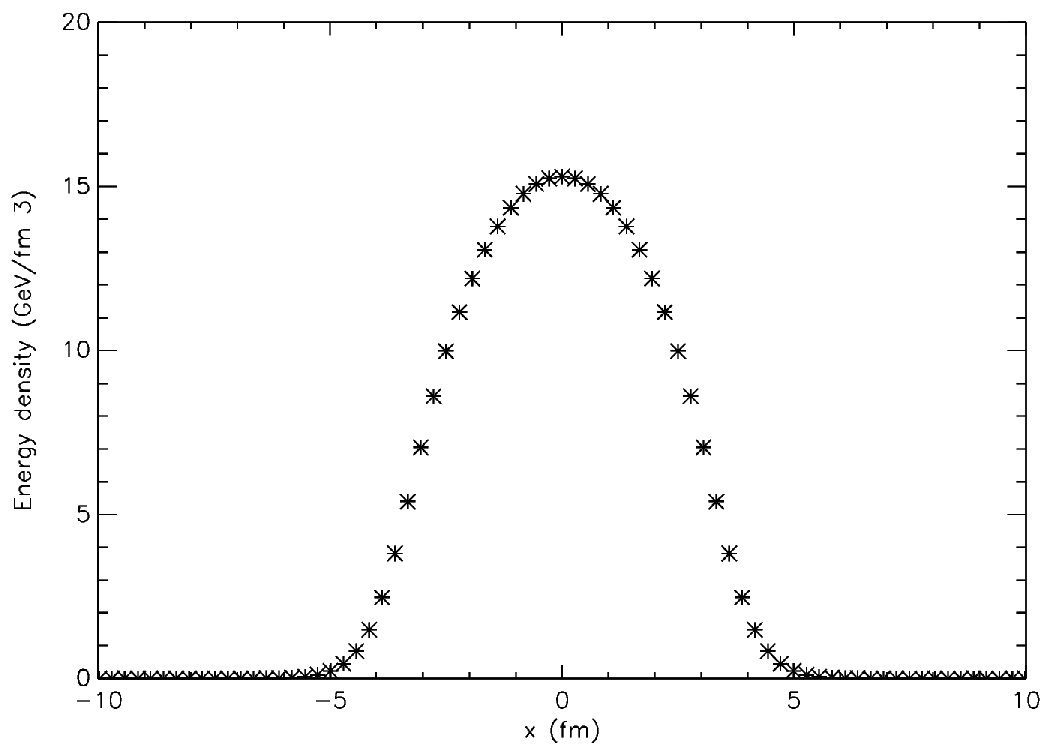
\includegraphics[width=8cm]{images/plot1.pdf}
   \caption{Plot of energy density in $GeV/fm^3$ at $\tau=1\,fm/c$ for $y=\eta=0$.}
    \label{plot1}
% \end{center}
\end{figure}

If we didn't plot the x array together with the \emph{en} slice, then gdl on the x axis would have used only the index numbers of the elements of the slice of the \emph{en} array.\\
Let's see now how the energy density profile looks like moving along the $\eta$ direction at x=y=0 (Fig. \ref{fig:plot2}):
\begin{lstlisting}[language=, numbers=none]
GDL> plot, z, en(50,50,*), xtitle="eta", ytitle="Energy density (GeV/fm^3)", xrange=[-10,10]
\end{lstlisting}
\begin{figure}[!h]
 \begin{center}
  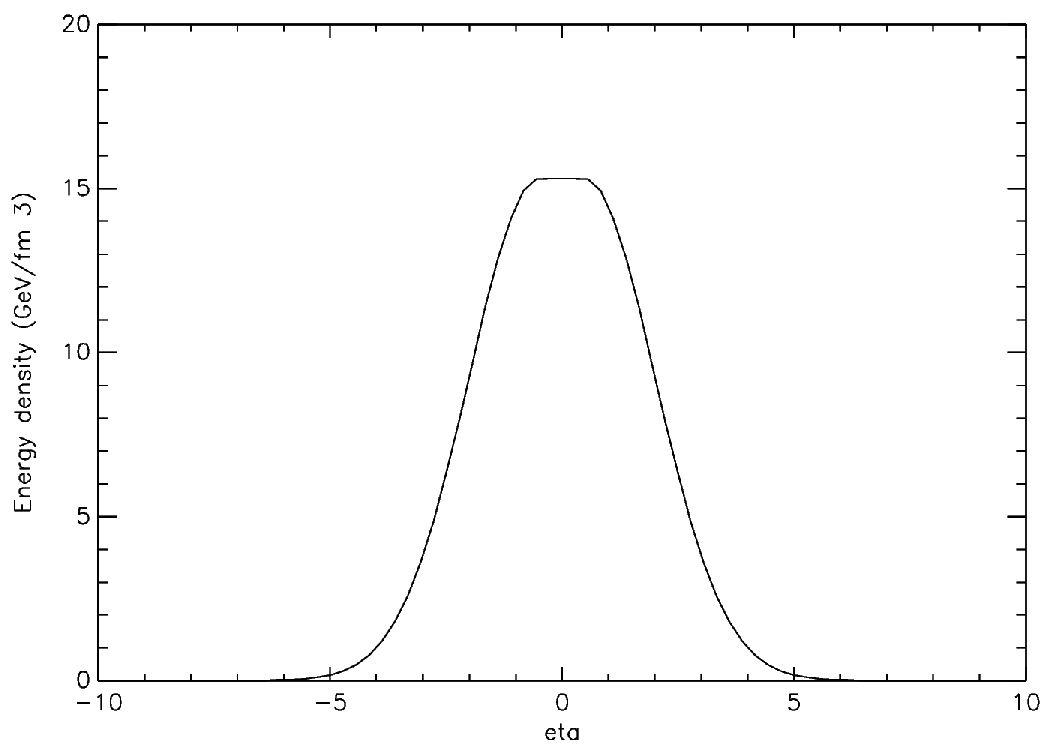
\includegraphics[width=8cm]{images/plot2.pdf}
   \caption{Plot of energy density in $GeV/fm^3$ at $\tau=1\,fm/c$ for $x=y=0$.}
    \label{fig:plot2}
 \end{center}
\end{figure}
Now let's make a surface plot of the energy density along the $x-\eta$ plane for $y=0$  (Fig. \ref{plot3}):
\begin{lstlisting}[language=, numbers=none]
GDL> surface, reform(en(*,50,*)), x, z, xtitle="x (fm)", ytitle="eta", ztitle="En. dens. (GeV/fm^3)", xrange=[-10,10], yrange=[-10,10]
\end{lstlisting}
\begin{figure}[!h]
 \begin{center}
  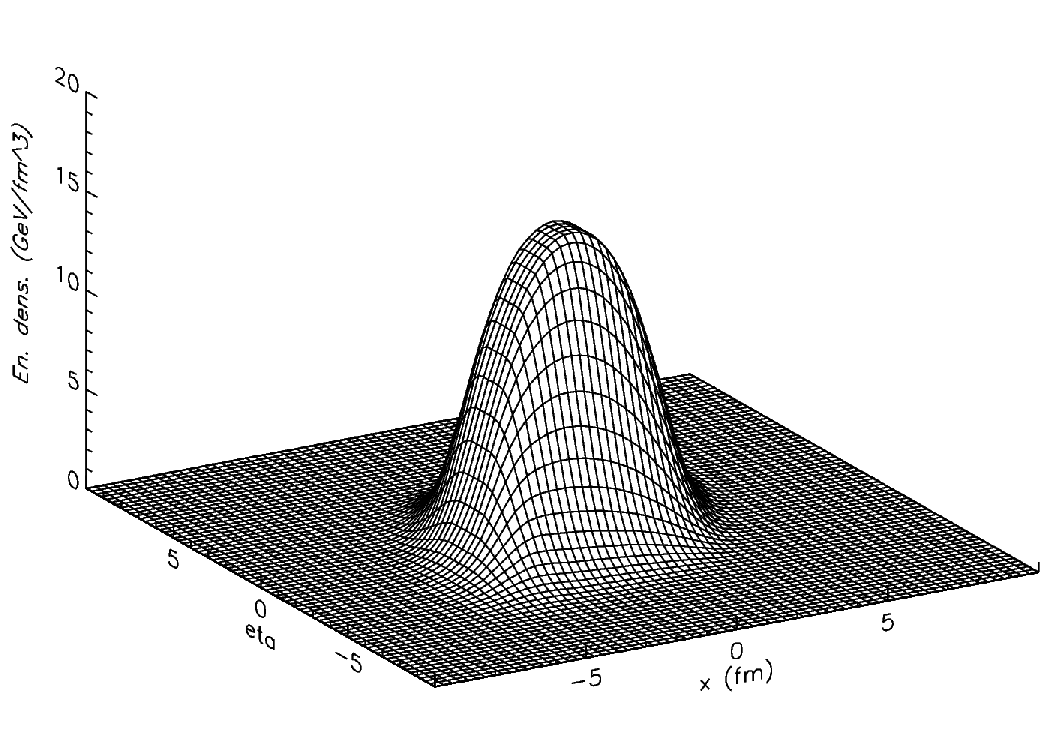
\includegraphics[width=8cm]{images/plot3.pdf}
   \caption{Surface plot of energy density in $GeV/fm^3$ at $\tau=1\,fm/c$ for $y=0$.}
    \label{plot3}
 \end{center}
\end{figure}
Let's replot the same quantities, but using a contour plot (Fig. \ref{plot4}):
\begin{lstlisting}[language=, numbers=none]
GDL> set_plot, 'ps'
GDL> device, filename="plot4.ps"
GDL> contour, reform(en(*,50,*)), x, z, xtitle="x (fm)", ytitle="eta", xrange=[-6,6],yrange=[-5,5], LEVELS = [0.0, 2.5, 5., 7.5, 10., 12.5, 15, 17.5, 20.], C_LABELS = [1, 0, 1, 0, 1, 0, 1, 0, 1]
GDL> device, /close
\end{lstlisting}
\begin{figure}[!h]
 \begin{center}
  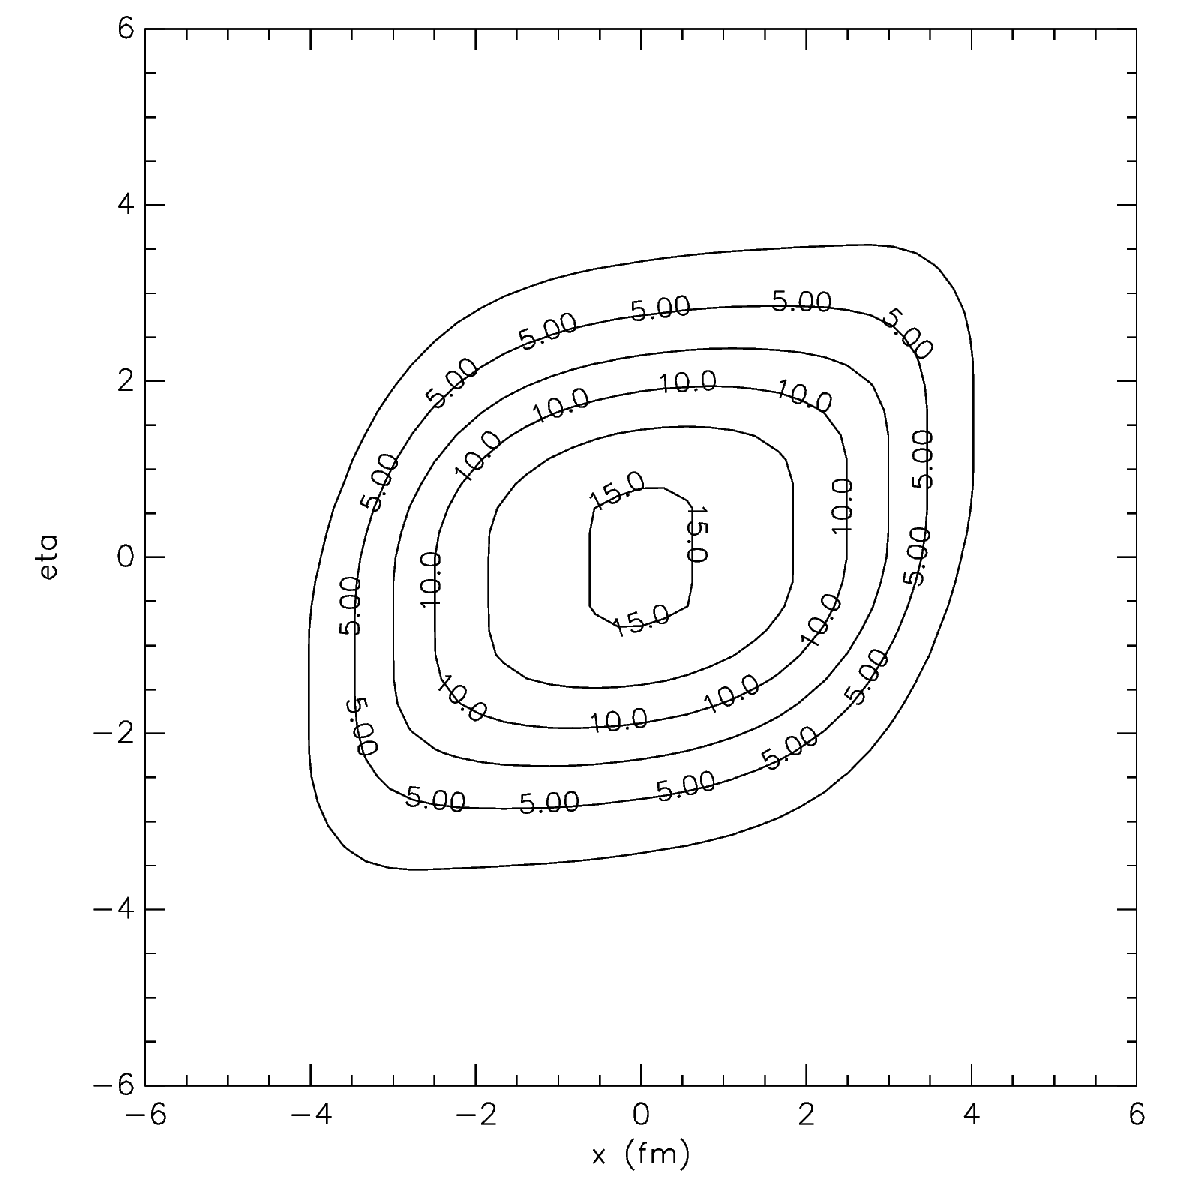
\includegraphics[width=8cm]{images/plot4.pdf}
   \caption{Contour plot of energy density in $GeV/fm^3$ at $\tau=1\,fm/c$ for $y=0$.}
    \label{plot4}
 \end{center}
\end{figure}
Now, let's have a look at what is the situation at a later time, using the fortran utilities.\\
Output data are written into binary files; the \emph{readx.exe} utility extracts these data into separate files for each variable in ascii format.\\
Calling readx.exe without any argument prints an help message:\\
\begin{lstlisting}[language=, numbers=none]
./readx.exe 
 Please, insert the range of echo-qgp output files from which you want to extract values.
 (Optionally, you can also write the name of the directory where the output files will be written)
 (default: postproc/readx) 
\end{lstlisting}
If we are interested only in output at $\tau=10.0\,fm/c$, we can look at the time.dat file and, after reading that corresponding output data number is 91, we can type:\\
\begin{lstlisting}[language=, numbers=none]
./readx.exe 91 91
  time=   9.9999999999999822
\end{lstlisting}
If we wished to extract all output data from $\tau=4.5\,fm/c$ to $\tau=4.8\,fm/c$ we would use:\\
\begin{lstlisting}[language=, numbers=none]
./readx.exe 36 39
  time=   4.5000000000000009     
  time=   4.6000000000000005     
  time=   4.7000000000000002     
  time=   4.7999999999999998  
\end{lstlisting}
Now, we copy the utility fromecho.exe into the new created postproc/readx directory and then we enter into it:\\
\begin{lstlisting}[language=, numbers=none]
cp fromecho.exe postproc/readx
cd postproc/readx
\end{lstlisting}
Calling \emph{fromecho.exe} without any arguments prints an help message:
\begin{lstlisting}[language=,numbers=none]
./fromecho.exe 
 Synopsis:
 To extract data from the left to the right border of the grid along x, y or z direction:
 ./fromecho input_file output_file x|y|z
 To extract data using a specific range along one direction and fixing the other ones at a point:
 ./fromecho input_file output_file x|y|z x-indx-start x-indx-end y-indx-start y-indx-end z-indx-start z-indx-end
 Please, note that starting and ending indexes of the fixed directions must be equal
 Usage example: ./fromecho prova_input prova_output y 33 33 2 150 44 44
 This extracts data from file prova_inputs and write the values along y direction from point with index 2 to
 point with index 150, fixing x at index 33 and z at index 44
\end{lstlisting}
We extract the value of temperature at $\tau=10\,fm/c$ along the x axis for $y=\eta=0$:
\begin{lstlisting}[language=, numbers=none]
./fromecho.exe T0091.dat temperature_x_tau_10.0.dat x 
\end{lstlisting}
Now extract the value of temperature at $\tau=10\,fm/c$ along the $\eta$ axis for $x=y=0$, for all the $\eta$ range (reminding that now indexes go from 1 to 101):
\begin{lstlisting}[numbers=none]
./fromecho.exe T0091.dat temperature_z_tau_10.0.dat z 51 51 51 51 1 101
\end{lstlisting}
All the files created by fromecho.exe consists of two columns: the first one is the coordinate position, the second one the value of the variable. This data format can be easily read by many plotting software.\\
For example, using gnuplot (Fig. \ref{plot4}):
\begin{lstlisting}[language=, numbers=none]
gnuplot
	G N U P L O T
	Version 4.6 patchlevel 0    last modified 2012-03-04 
	Build System: Linux x86_64

	Copyright (C) 1986-1993, 1998, 2004, 2007-2012
	Thomas Williams, Colin Kelley and many others

	gnuplot home:     http://www.gnuplot.info
	faq, bugs, etc:   type "help FAQ"
	immediate help:   type "help"  (plot window: hit 'h')

Terminal type set to 'wxt'
gnuplot> set term pos eps col enh font "Helvetica, 22"
Terminal type set to 'postscript'
Options are 'eps enhanced defaultplex \
   leveldefault color colortext \
   dashed dashlength 1.0 linewidth 1.0 butt noclip \
   nobackground \
   palfuncparam 2000,0.003 \
   "Helvetica" 22  fontscale 1.0 '
gnuplot> set out "temperature.eps"
gnuplot> set ylabel "Temperature (GeV)"
gnuplot> set xlabel "{/Symbol h}"
gnuplot> plot "./temperature_z_tau_10.0.dat" with linespoints lt 7 linecolor 3 notitle
\end{lstlisting}
We remind that the image files in Encapsulated Postscript (.eps) format can be converted into Portable Document Format (.pdf) with the utility ps2pdf, e.g.:
\begin{lstlisting}[numbers=none, language=]
ps2pdf -dEPSCrop temperature.eps
\end{lstlisting}

\begin{figure}[!h]
 \begin{center}
  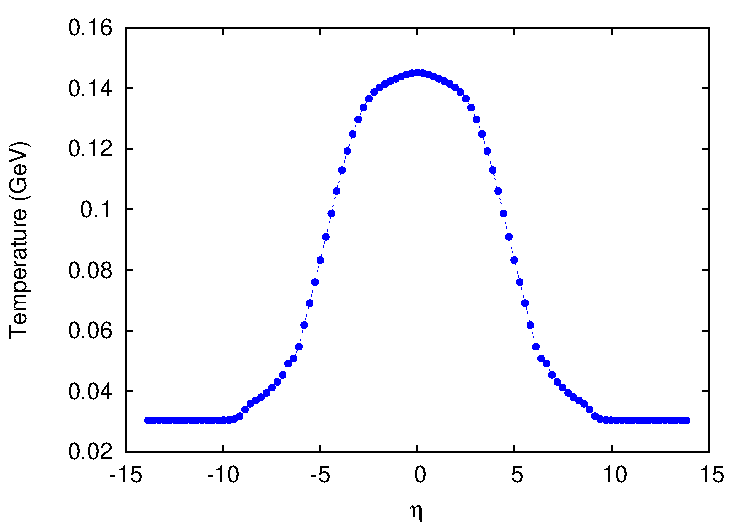
\includegraphics[width=8cm]{images/temperature.pdf}
   \caption{Test A - Temperature profile at $\tau=10\,fm/c$ for $y=\eta=0$.}
    \label{plot4}
 \end{center}
\end{figure}
We can use the utility \emph{fromecho2d.exe} to extract values for a 2D slice of the grid, for example:
\begin{lstlisting}[language=, numbers=none] 
 ./fromecho2d.exe T0091.dat tempxz91.dat x z
\end{lstlisting}
Then, we can use a gnuplot script like the following to plot the data:
\begin{lstlisting}[numbers=none, language=Gnuplot]
# Set terminal and output
set terminal pngcairo size 900, 900 enhanced font 'Helvetica,22'
set encoding utf8
set output 'contour91xz.png'

# Set plot properties
set size square
set pm3d
unset surface 
set view map
set key outside
set pm3d interpolate 0,0 # interpolate the color

# Set the color palette
set palette model RGB defined ( 0 'black', 1 'blue', 2 'cyan' ,3 'green' ,4 'yellow', 5 'red', 6 'purple' )

# Se the axes
set xlabel 'x (fm)'
set ylabel "{/Symbol h}"
set cblabel "Temperature (MeV)"

# Draw the plot
splot 'tempxz91.dat' u 1:2:($3*1000.) notitle
\end{lstlisting}
\begin{figure}[!h]
 \begin{center}
  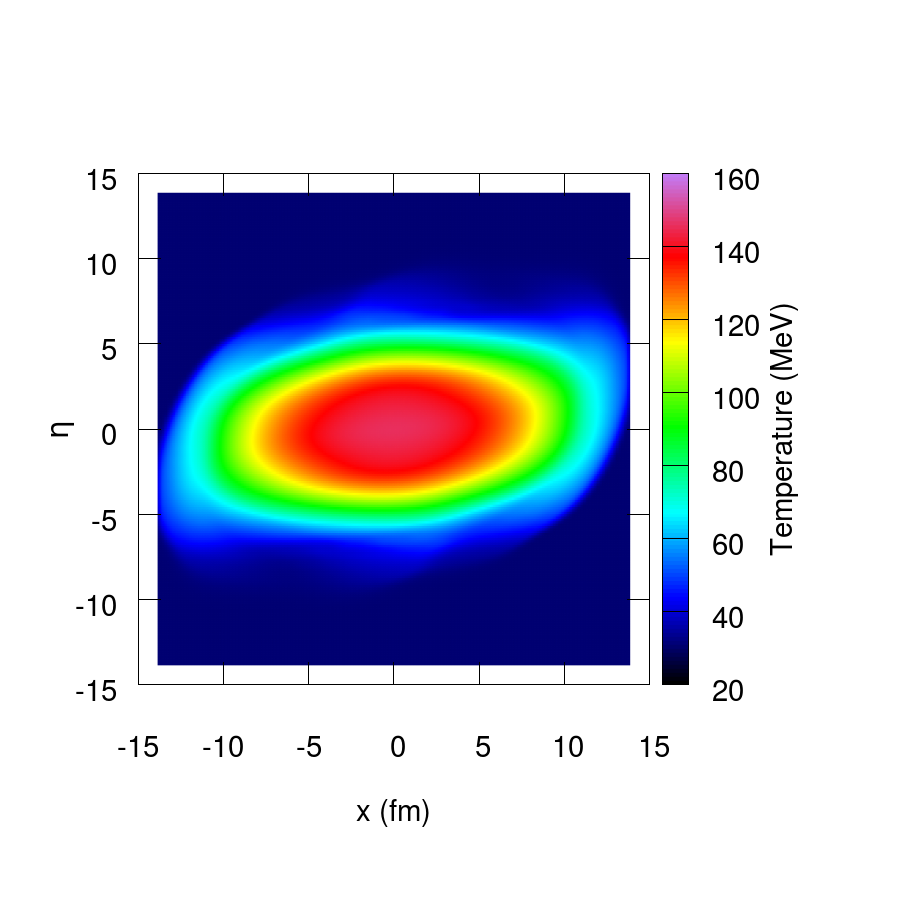
\includegraphics[width=8cm]{images/contour91xz.png}
   \caption{Test A - Contour of temperature (MeV) at $\tau=10\,fm/c$ for $y=0$.}
    \label{plot5}
 \end{center}
\end{figure}
A copy of the plotted datafile {\tt tempxz91.dat} can be found in {\tt tests/testA}.\\
Now let's see how to compute the thermal particle spectra.\\
From the ECHO-QGP main directory of sources we enter the {\tt analysis} subdirectory and we compile the tools:
\begin{lstlisting}[numbers=none]
make
\end{lstlisting}
We remind that, to make use of OPENMP, the user has to edit the makefile and export some environment variable, see \ref{spectra-comp} for more details.
Using the following configuration file {\tt settings.txt}:
\begin{lstlisting}[numbers=none]
! This is the file containg the settings for the routine producing the spectra 
! *** ECHO-RELATED
dim......=3                               ! 1+1, 2+1, 3+1 dimension for the simulation
visco_hyd=1                               ! Is it a viscous hydro simulation?  0=no, 1=yes
visco_spe=1                               ! viscosity corrections to the distribution function? 0=no, 1=yes
vorticity=0                               ! Evaluate vorticity on hypersurface
nout.....=0                               ! total number of outputs (if 0 reads all available)
! *** PARTICLE-RELATED
npt......=40                              ! points for the transverse momentum
ptmin....=0.0                             ! min transverse momentum
ptmax....=4.0                             ! max transverse momentum
nphi.....=36                              ! points for the polar angle 
phimin...=0.0                             ! min polar angle 
phimax...=6.28318530718                   ! max polar angle 
nrap.....=41                              ! points for the particle rapidity 
rapmin...=-4.0                            ! min rapidity
rapmax...=4.0                             ! max rapidity 
listorseq=2                               ! 0- all; 1-sequence ID_start-ID_stop; 2-list; 3-stable
ID_start.=211                             ! ID of first particle to be considered
ID_stop..=-10213                          ! ID of last particle to be considered
part_list=2                               ! particles in the list 
211
3122
antibar..=1                               ! 1=on 0=off
chempot..=1                               ! read chemical potential from ../eos_data/chemical_potential.txt; 0 ste mu=0
! *** INPUT 
inputdir.=../outr0001/                    ! input directory 
ioutdir..=../outr0001/spectra/            ! output directory
file.....=out                             ! name of the ECHO outout file
! *** RANDOM SEED (saved anyway)
seed.....=0                               ! if 0 generates random seed, otherwise use that
ptbox....=3.0                             ! upper limit for mc box
phibox...=0                               ! if 0 is 2*pi
ybox.....=00.0                            ! upper limit for mc box
! *** HISTOGRAM-RELATED
mxv_pt...=3.0                             ! max value for pt
mnv_pt...=0.0                             ! min value for pt
mxv_ang..=6.28318                         ! max value for phi
mnv_ang..=0.0                             ! min value for phi
mxv_y....=0.0                             ! max value for y
mnv_y....=-0.0                            ! min value for y
binpt....=50                              !
binphi...=1                               !
binrap...=1                               !
6.28318530718
\end{lstlisting}
we can compute the thermal spectra of $\pi^+$, $\Lambda^0$ and $\overline{\Lambda^0}$, taking into account the viscous corrections to the distribution function.\\
Please, remember to create the {\tt outr0001/spectra} directory before running the tool.\\
After executing the program:
\begin{lstlisting}[numbers=none, language=]
./thermal.exe
\end{lstlisting}
we can enter into {\tt outr0001/spectra} and make some plots:
\begin{lstlisting}[numbers=none, language=]
gnuplot plot_pionplus_spectra.gp
\end{lstlisting}
The plot files can be quickly converted from EPS to PDF with
\begin{lstlisting}[numbers=none, language=BASH]
for i in *.eps; do ps2pdf -dEPSCrop $i; done
\end{lstlisting}
(See figures \ref{plotdNdy},\ref{plotI},\ref{plotv1},\ref{plotv2}).
\begin{figure}[!h]
 \begin{center}
  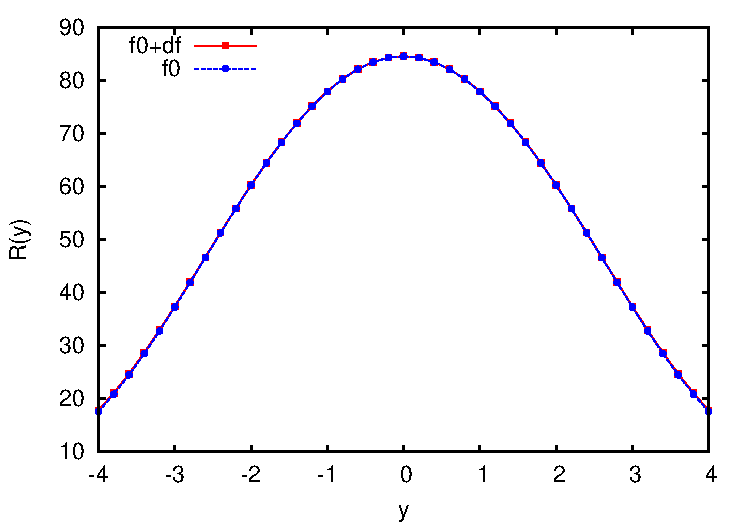
\includegraphics[width=8cm]{images/dNdy_pi_plus.pdf}
   \caption{Test A - $dNdy$ of $\pi^+$ particles. Red color means that viscous corrections to thermal distribution have been taken into account, blue color means not.}
    \label{plotdNdy}
 \end{center}
\end{figure}
\begin{figure}[!h]
 \begin{center}
  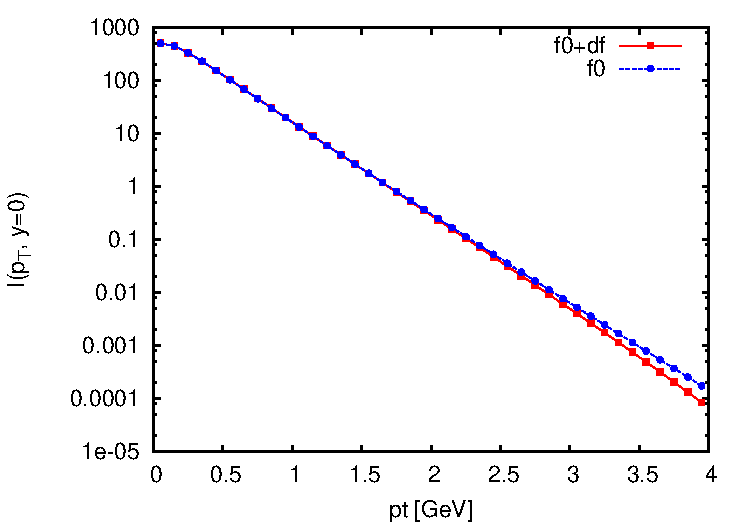
\includegraphics[width=8cm]{images/spectra_pi_plus.pdf}
   \caption{Test A -  $I(p_T,y=0)$ of $\pi^+$ particles. Red color means that viscous corrections to thermal distribution have been taken into account, blue color means not.}
    \label{plotI}
 \end{center}
\end{figure}
\begin{figure}[!h]
 \begin{center}
  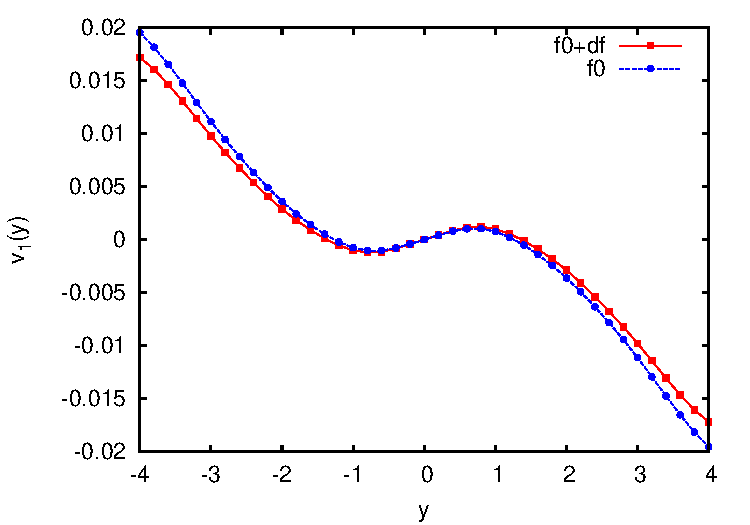
\includegraphics[width=8cm]{images/v1_pi_plus.pdf}
   \caption{Test A -  Directed flow of $\pi^+$ particles. Red color means that viscous corrections to thermal distribution have been taken into account, blue color means not.}
    \label{plotv1}
 \end{center}
\end{figure}
\begin{figure}[!h]
 \begin{center}
  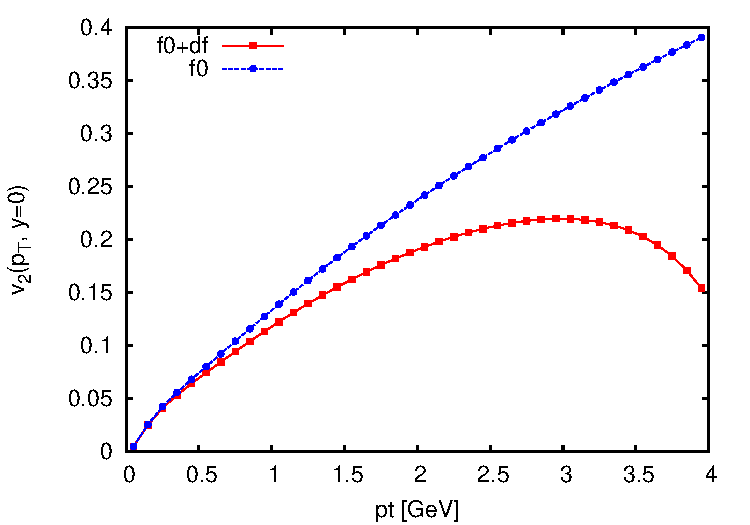
\includegraphics[width=8cm]{images/v2_pi_plus.pdf}
   \caption{Test A -  Elliptic flow of $\pi^+$ particles. Red color means that viscous corrections to thermal distribution have been taken into account, blue color means not.}
    \label{plotv2}
 \end{center}
\end{figure}
\section{2D shock tube - test B}
This is a simple test of a 2D shock wave.\\
The param.dat files of this test can be found into the {\tt tests/testB directory}.\\
The initial state is simply costitued by a sharp jump in pressure when crossing the $y=-x$ locus, whose values can be adjusted editing the {\tt init.f90} file a few lines after the condition:
\begin{lstlisting}[numbers=none, language=]
else if ( init_type .eq. SHOCK_TUBE_2D) then
\end{lstlisting}
\begin{lstlisting}[numbers=none, language=Fortran]
if(y(iy) .lt. -x(ix)) then
   vv(kpr)=5.401411
else
   vv(kpr)=0.337588
end if
\end{lstlisting}
After compiling ECHO-QGP, we run ECHO-QGP a few times using different values for $\eta/s$, changing the ETA\_S parameter into {\tt param.dat}. We can also execute an inviscid simulation setting the parameter VISCOUS..=0. Please, take care to not overwrite the results of the various simulations, either renaming the output directory after the end of each simulation or using the \emph{-o} flag when launching the program (e.g. \emph{./echo.exe -o out\_2Dtest}).\\
First, we check if the initial conditions are correct.\\
We copy the {\tt tools/readvar.pro} gdl script into the output directory (e.g. {\tt outr0001}, but it could have a different name) and then we use it:\\
\begin{lstlisting}[numbers=none, language=]
cd outr0001
gdl
\end{lstlisting}
\begin{lstlisting}[numbers=none, language=]
GDL> readvar, 0001
\end{lstlisting}
We can make a sketchy plot simply typing:
\begin{lstlisting}[numbers=none, language=]
GDL> plot, x, pr(*,100)
\end{lstlisting}
This is fine to make a simple check, but, if we wish to prepare a better quality plot, we can export the data to a file and then use it another tool (e.g. gnuplot, grace and many others). To perform this task, we can use the fortran postprocessing tools or gdl itself, preparaing, for example, a script like (file {\tt tests/testB/tofile.pro}):
\begin{lstlisting}[numbers=none, language=IDL]
openw, 12, "initial_pressure_testB.dat" 

;please, change the for-cycle interval accordingly with your grid
;remind that array indexes in gnudatalanguage start from 0
;for example, if you have a 201x201 grid, initial and final values are 0 and 200
;and, if the grid is symmetric respect to the origin, the index corresponding to 0 is 100
for i=0,200 do begin
        printf, 12, x(i), pr(i,100)
endfor

free_lun, 12

END 
\end{lstlisting}
If we run the script with:
\begin{lstlisting}[numbers=none, language=]
GDL> .r tofile
\end{lstlisting}
we should get an ascii file called {\tt initial\_pressure\_testB.dat} which we can plot using another program (\ref{testB_init_pressure}):
\begin{figure}[!h]
 \begin{center}
  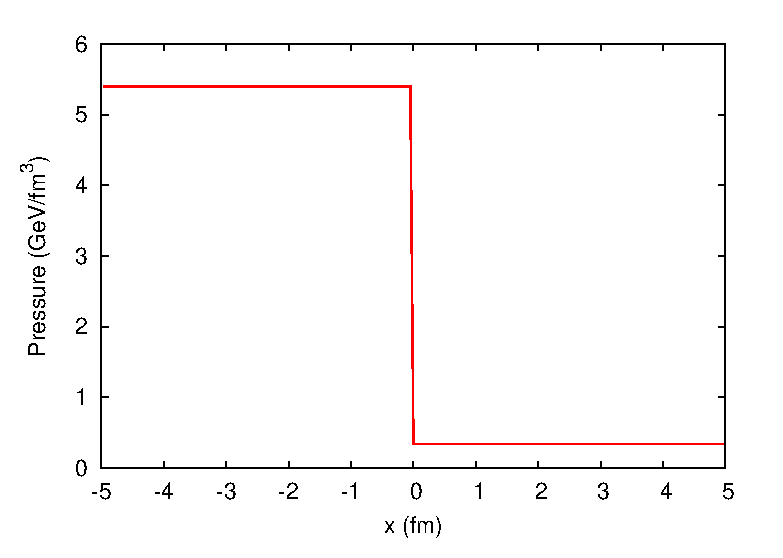
\includegraphics[width=8cm]{images/initial_pressure_testB.eps}
   \caption{Test B - Initial pressure profile at $\tau=1,fm/c$ for $y=0$.}
    \label{testB_init_pressure}
 \end{center}
\end{figure}
Assuming to have executed four simulations, one inviscid and the other three with $\eta/s=0.001,\,0.01,\,0.1$, after compiling the fortran tools and copying them into the output directory, we can extract the data at the end of the run ($\tau=4$ fm/c) with:
\begin{lstlisting}[numbers=none, language=]
./readx.exe 31 31
\end{lstlisting}
followed by (into the postproc/readx directory):
\begin{lstlisting}[numbers=none, language=]
./fromecho.exe EPS0031.dat en0_1.dat x 1 201 101 101 1 1 
./fromecho.exe VX0031.dat vx0_1.dat x 1 201 101 101 1 1
\end{lstlisting}
In the previous example, the name of the output files refer to energy density and $V_x$ of the run with $\eta/s=0.1$.\\
In the {\tt tests/testB} directory there is a simple gnuplot script to plot the results after gathering them in a common directory (Fig. \ref{testB_final_velocity} and \ref{testB_final_energy_density}).\\
\begin{figure}[!h]
 \begin{center}
  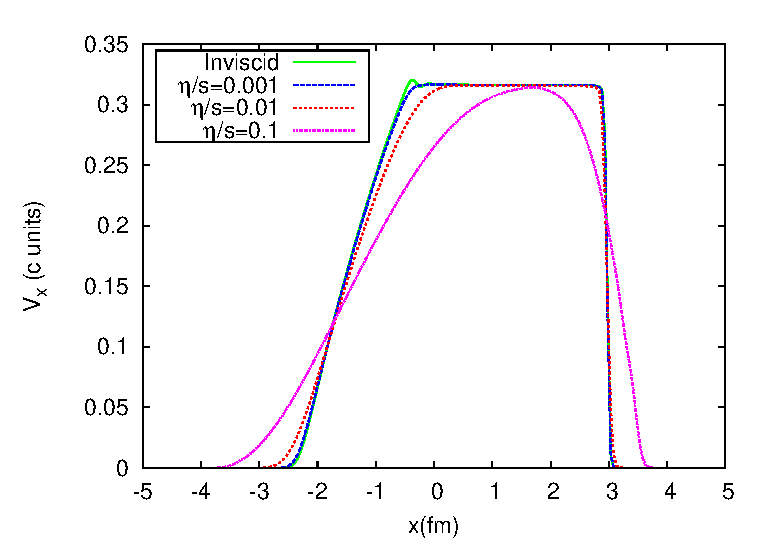
\includegraphics[width=8cm]{images/vx-comparison-testB.eps}
   \caption{Test B - Comparison of $V_x$ profiles at $\tau=4,fm/c$ for $y=0$.}
    \label{testB_final_velocity}
 \end{center}
\end{figure}
\begin{figure}[!h]
 \begin{center}
  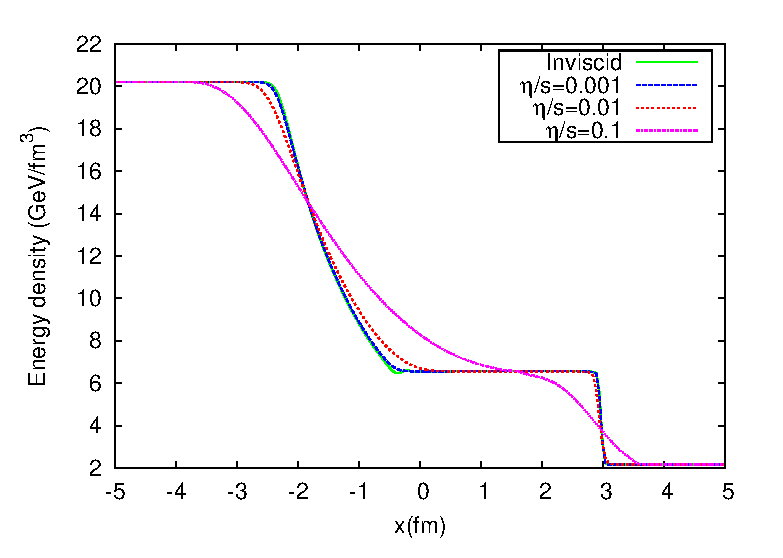
\includegraphics[width=8cm]{images/en-comparison-testB.eps}
   \caption{Test B - Comparison of energy density profiles at $\tau=4,fm/c$ for $y=0$.}
    \label{testB_final_energy_density}
 \end{center}
\end{figure}

\section{1D viscous shear flow test - test C}\label{sec:gub}
This is merely the execution of the test described in section \ref{test1D} and \cite{DelZanna:2013eua}.\\
The file {\tt param.dat} to set up the simulation can be found in {\tt tests/testC}.\\
The results can be examined with the usual tools, following the procedures already shown in the previous examples:\\
\begin{lstlisting}[numbers=none, language=]
./readx.exe 91 91
./fromecho.exe VY0091.dat vy.dat x 1 301 1 1 1 1
\end{lstlisting}
A simple gnuplot script ({\tt plot1D.gp}) to plot the results is also included.\\
\begin{figure}[!h]
 \begin{center}
  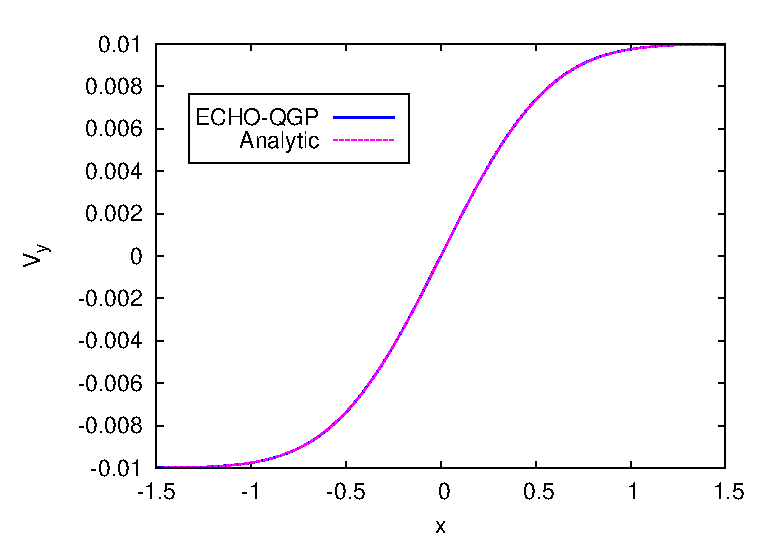
\includegraphics[width=8cm]{images/test1D.eps}
   \caption{Test C - Comparison between the analytical solution and ECHO-QGP at $\tau=10$ fm/c.}
    \label{testC}
 \end{center}
\end{figure}

\section{Gubser flow test - test D}
The description of this test can be found on \cite{Marrochio:2013wla} \cite{Becattini:2015ska}, here we'll simply summarize what do to perform it.\\
First, we need a set of initial values, which can be found into the {\tt tests/testD} directory. This file, named {\tt Initial\_Profile\_GubserFlow.dat}, has been produced with \emph{Maple 12} executing the worksheet {\tt initial\_conditions\_maple12.mw} contained into the same directory.
The settings inside param.dat must match those of the tabulated initial conditions (e.g. the grid) and also $\tau_{\pi}$, $\eta/s$ and the relation between temperature and energy density must correspond to what chosen for computing the input file with initial conditions. The file {\tt tests/testD/param.dat} works with the provided intial conditions.\\
To complete the setup, the user has to comment/uncomment the temperature relation with energy density inside the eos\_data/temperature.def file, clean the sources with \emph{make clean} and recompile ECHO-QGP. If the grid used for computing the initial conditions is changed, then it is required to change not only the lines defining the grid into param.dat, but also the checks contained into {\tt init.f90} after the line with comment ``! GUBSERCHECKS''.\\
Since in this test we wish to compare the evolution of some variables with the semianalytical solutions obtained numerically with some external code, we need also these solutions. In the {\tt tests/testD} directory we provide the solutions computed with \emph{Maple 12} at $\tau=4$ fm/c; the Maple worksheet can be reused, with only minor changes, to compute the solutions at different times and/or with different grid resolutions.\\
After the end of the run, we can check the results. There are many ways to do it, here we'll use gdl and gnuplot.\\
\begin{lstlisting}[numbers=none, language=]
cd outr0001
\end{lstlisting}
\begin{lstlisting}[numbers=none, language=]
gdl
\end{lstlisting}
We can use the shell commands inside \emph{gnudatalanguage} adding a dollar (\$) sign before issuing the command. For example, to list the files inside the current directory to check if the script {\tt readvar.pro} is there we can type:
\begin{lstlisting}[numbers=none, language=]
GDL> $ls -l | grep readvar
-rw-r--r-- 1 g g    12562 mag  9 02:42 readvar.pro
\end{lstlisting}
Now we read the output at $\tau=4$ fm/c (please, remind that you can look at {\tt time.dat} to see what is the output number corresponding to that time).
\begin{lstlisting}[numbers=none, language=]
GDL> readvar, 0031
% Compiled module: READVAR.
This program reads the output of echo-qgp
Reading grid_summary.dat
nx   :      401
ny   :      401
nz   :        1
xstep:     0.0500000  - ystep:     0.0500000  - zstep:       2.00000
xmin:      -10.0250  - ymin:      -10.0250  - zmin:      -1.00000
xmax:       10.0250  - ymax:       10.0250  - zmax:       1.00000
Reading grid.dat
% Compiled module: SKIP_LUN.
Run with viscosity
Output has        8 bytes precision
Variables to be read:
density
vx
vy
vz
pressure
energy density
temperature
entropy density
bulk viscosity
pi^tt
pi^tx
pi^ty
pi^tz
pi^xy
pi^xz
pi^yz
pi^xx
pi^yy
pi^zz
gamma
Number of variables is:       20
Reading file: out0031.dat
time : 4.00000000  
time (or tau) is stored into variable t=       4.0000000
Arrays available: x,y and z of type double with      401     401       1 elements
Arrays available with their maximum, mean and minimum values:
% Compiled module: MEAN.
rho:      0.21052070      0.12870059    0.0034551016
vx:      0.97009619   8.2463097e-16     -0.97009619
vy:      0.97009619  -6.2895014e-15     -0.97009619
vz:       0.0000000       0.0000000       0.0000000
pr:    0.0074253124    0.0010125367   1.0013452e-05
en:     0.022275937    0.0030376102   3.0040355e-05
temp:     0.059237610     0.027047653     0.011351802
entropy:      0.50139177     0.088629927    0.0035284097
bu:       0.0000000       0.0000000       0.0000000
tt:       0.0000000   -0.0011994727   -0.0089583879
tx:    0.0093095075  -3.2743781e-18   -0.0093095075
ty:    0.0093095075  -6.1862789e-18   -0.0093095075
tz:       0.0000000       0.0000000       0.0000000
xy:    0.0044716459   1.7072896e-18   -0.0044716459
xz:       0.0000000       0.0000000       0.0000000
yz:       0.0000000       0.0000000       0.0000000
xx:   1.1768752e-05  -0.00081962219   -0.0096843503
yy:   1.1768752e-05  -0.00081962219   -0.0096843503
zz:   0.00010049364   2.7411661e-05  -3.8899064e-07
v0:       4.1203721       1.9250202       1.0000000
\end{lstlisting}
Now we read the tabulated file with the solutions computed by Maple using the script {\tt read\_M12.pro}, in the {\tt tests/testD} directory:
\begin{lstlisting}[numbers=none, language=]
GDL> .r read_M12
% Compiled module: $MAIN$.
mx12,my12,mtemp12,mux12,muy12,mpixx12,mpiyy12,mipxy12,mpitt12,mpitx12,mpity12,mpizz12
\end{lstlisting}
The script reads the file {\tt maple\_gub\_full\_y\_eq\_x\_tau\_4.0}; the user can easily modify the worksheet to read other files with the same structure.\\
Now we prepare the data for plotting. We are interested in the values with coordinates $x=y$, so first we declare an array to store these values:
\begin{lstlisting}[numbers=none, language=IDL]
GDL> a=dblarr(401)
\end{lstlisting}
Then we fill the array, in this example with the values of $u^x=\gamma v^x$:
\begin{lstlisting}[numbers=none, language=IDL]
GDL> for i=0,400 do a(i)=v0(i,i)*vx(i,i)
\end{lstlisting}
And now we print the values to compare into the file {\tt ux-comparison.dat}:
\begin{lstlisting}[numbers=none, language=IDL]
GDL> openw, 12, "ux-comparison.dat"
GDL> for i=0,400 do printf, 12, x(i), a(i), mux12(i)
GDL> free_lun, 12
\end{lstlisting}
Now we can make the plot with gnuplot:
\begin{lstlisting}[numbers=none, language=Gnuplot]
set term pos eps col enh font "Helvetica,22"
set out "ux.eps"
set xlabel "x (fm)"
set ylabel "u^x (c units)"
set key top left box
plot "ux_comparison.dat" u 1:2 w l lt 1 lc 3 lw 3 title "ECHO-QGP", "ux_comparison.dat" u 1:3 w l lt 3 lc 4 lw 3 title "Semianalytic"
\end{lstlisting}
The commands are gathered into the {\tt plot-ux.gp} script under tests/testD, which can be executed with:
\begin{lstlisting}[numbers=none, language=]
gnuplot plot-ux.gp
\end{lstlisting}
\begin{figure}[!h]
 \begin{center}
  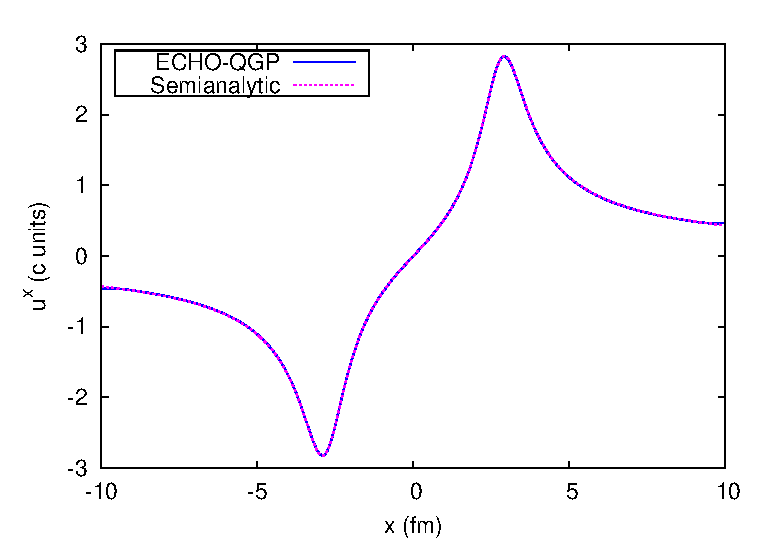
\includegraphics[width=8cm]{images/ux-testD.eps}
   \caption{Test D - Comparison between the semianalytical solution and ECHO-QGP results at $\tau=4$ fm/c.}
    \label{fig:testD1}
 \end{center}
\end{figure}
Into the {\tt tests/testD} directory there are a few more plots of other variables, obtained with the same procedure.\\
\section{Initialization with a tabulated file - test E}
In this kind of initialization, the initial entropy density distribution is provided with an ascii tabulated file.\\
Changing the IENENTR parameter from 1 to 0, it is also possible to initialize ECHO-QGP using an energy density distribution. The name of the input file can be chosen with the IN\_D\_FILE parameter.\\
The input file for this example is created with a short python script ({\tt init\_tab.py}) that computes a simple gaussian distribution. The script and the {\tt param.dat} file to configure ECHO-QGP are into the tests/testE directory. See figures \ref{fig:testE1} and \ref{fig:testE2}.\\
\begin{figure}[!h]
 \begin{center}
  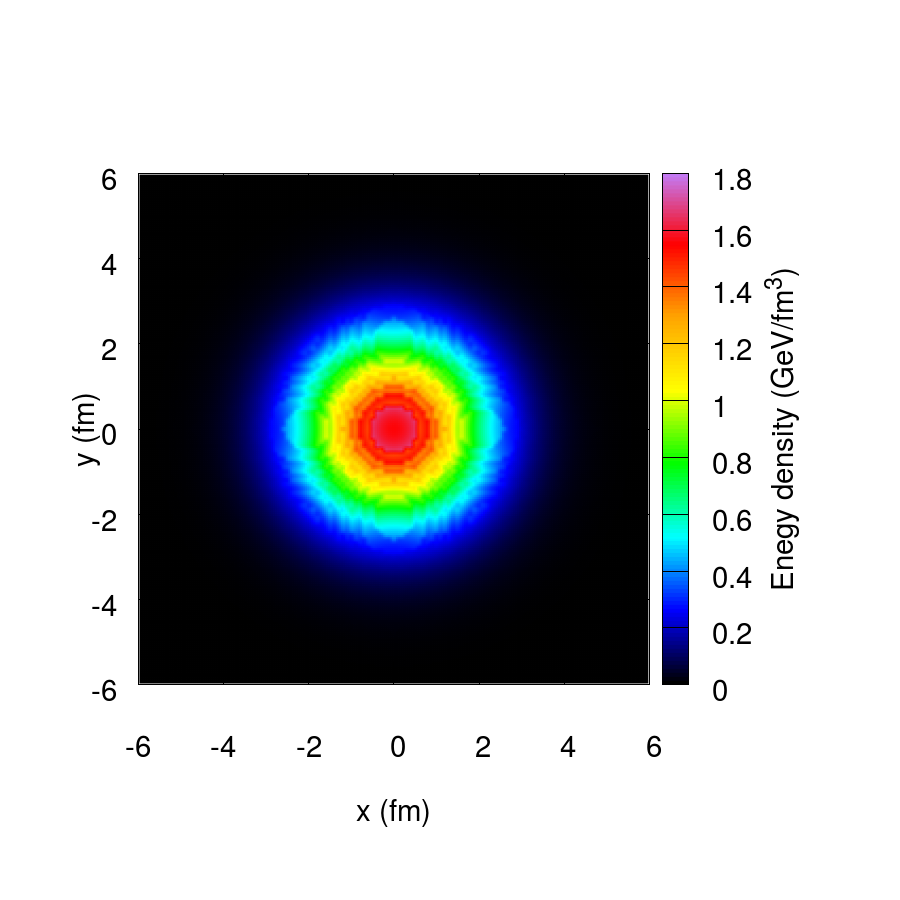
\includegraphics[width=8cm]{images/contour_energy_density_tau1.png}
   \caption{Test E - Initial energy density distribution at $\tau=1$ fm/c.}
    \label{fig:testE1}
 \end{center}
\end{figure}
\begin{figure}[!h]
 \begin{center}
  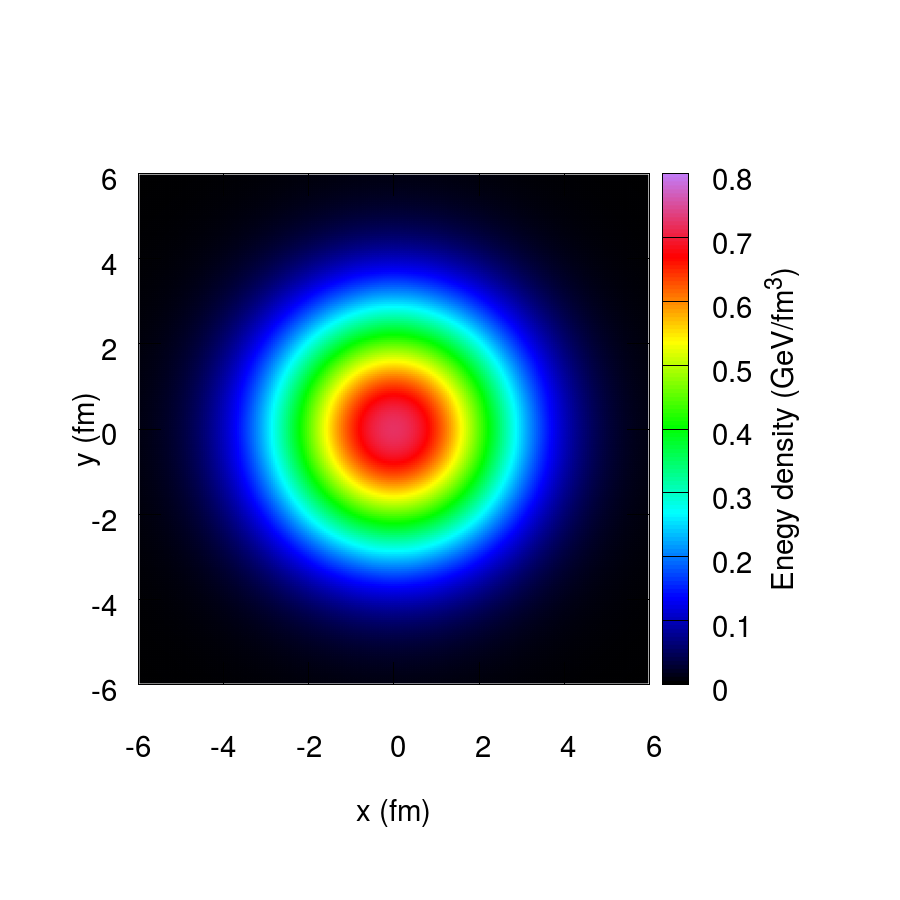
\includegraphics[width=8cm]{images/contour_energy_density_tau5.png}
   \caption{Test E - Energy density distribution at $\tau=5$ fm/c.}
    \label{fig:testE2}
 \end{center}
\end{figure}

\section{Glauber Monte Carlo initialization - test F}
In the {\tt tests/testF} directory can be found a {\tt param.dat} file to initialize a Glabuer-Monte Carlo simulation.\\
The random seed determines what will be the sequence of events, so, using the same random seed, saved into the file {\tt random\_seed.dat}, it is possible to reproduce the same initial series of events.\\
Other parameters can be ajdusted editing the first lines of {\tt glaubermc.f90}.\\
In this example, we try to produce a series of events from a sequence of 500 nuclear configurations, each with 20 different impact parameters, getting 1881 events which satisfy our selection criteria (i.e., a minimum of 18 participants, as specified with the option \emph{min\_participants=18} at the beginning of file {\tt glaubermc.f90}). The results are stored into the file {\tt partcoll.dat}. From this list, we select the event with id 67, but we can choose a sequence of events instead of a single one.\\
Now we plot the initial energy density distribution. The procedure, for each plot, is the same, apart, obviously, for the names of the files. For the event with id 67:\\
we compile the fortran prostprocessing tools:
\begin{lstlisting}[numbers=none, language=]
make tools
\end{lstlisting}
\begin{lstlisting}[numbers=none, language=]
cp tools/readx.exe outr0067
\end{lstlisting}
\begin{lstlisting}[numbers=none, language=]
cd outr0067
\end{lstlisting}
We are interested in the first and last output files, so:
\begin{lstlisting}[numbers=none, language=]
./readx 1 1
\end{lstlisting}
\begin{lstlisting}[numbers=none, language=]
./readx 94 94
\end{lstlisting}
\begin{lstlisting}[numbers=none, language=]
cp ../tools/fromecho*.exe postproc/readx
\end{lstlisting}
\begin{lstlisting}[numbers=none, language=]
cd postproc/readx
\end{lstlisting}
\begin{lstlisting}[numbers=none, language=]
./fromecho2d.exe EPS0001.dat en_out1.dat x y
\end{lstlisting}
\begin{lstlisting}[numbers=none, language=]
gnuplot contour_out1.gp
\end{lstlisting}
The Fig. \ref{fig:endens-gmc1} shows the initial energy distribution on the $\eta=0$ (x,y) plane at $\tau=1$ fm/c.
\begin{figure}[!h]
 \begin{center}
  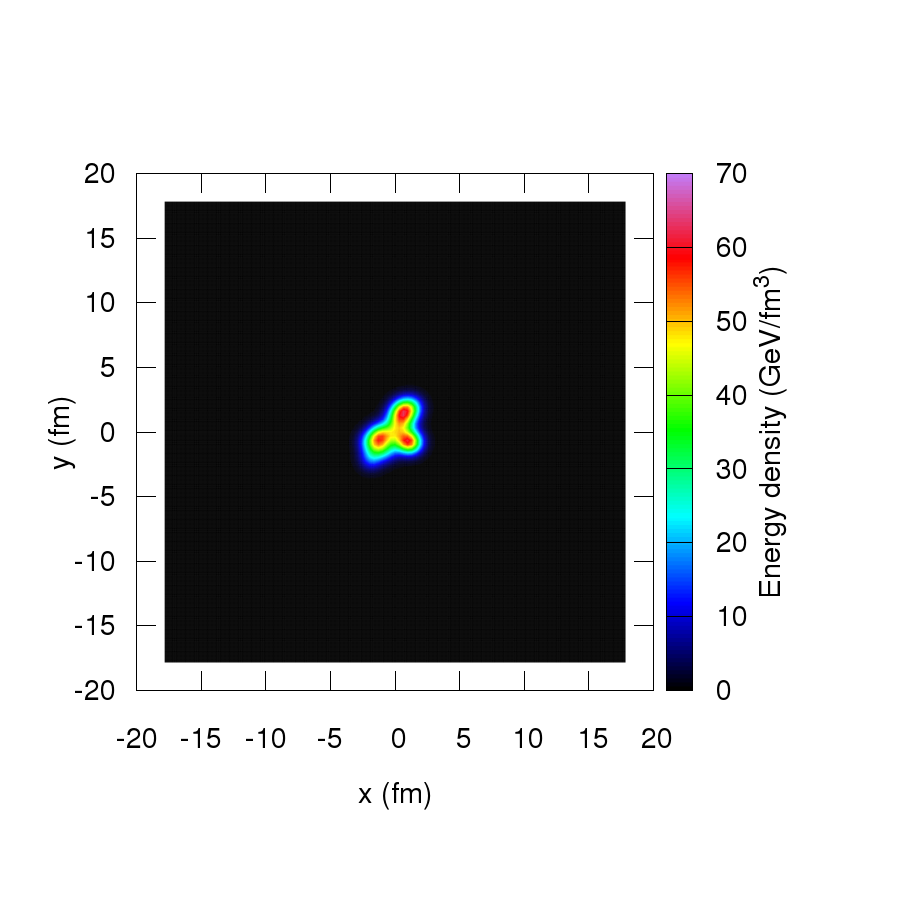
\includegraphics[width=8cm]{images/gmc_energy_density_contour_at_eta_0_tau1.png}
   \caption{Test F - Initial energy density distribution at $\tau=1$ fm/c with Glauber-MonteCarlo initialization.}
    \label{fig:endens-gmc1}
 \end{center}
\end{figure}
Now we look at the energy density profile as a function of $\eta$ for $x=y=0$ (Fig. \ref{fig:endens-gmc3}):
\begin{lstlisting}[numbers=none, language=]
./fromecho.exe EPS0001.dat energy_vs_eta_tau1.dat z 56 56 56 56 1 81
\end{lstlisting}
\begin{lstlisting}[numbers=none, language=]
gnuplot plot_en_vs_eta.gp
\end{lstlisting}
\begin{figure}[!h]
 \begin{center}
  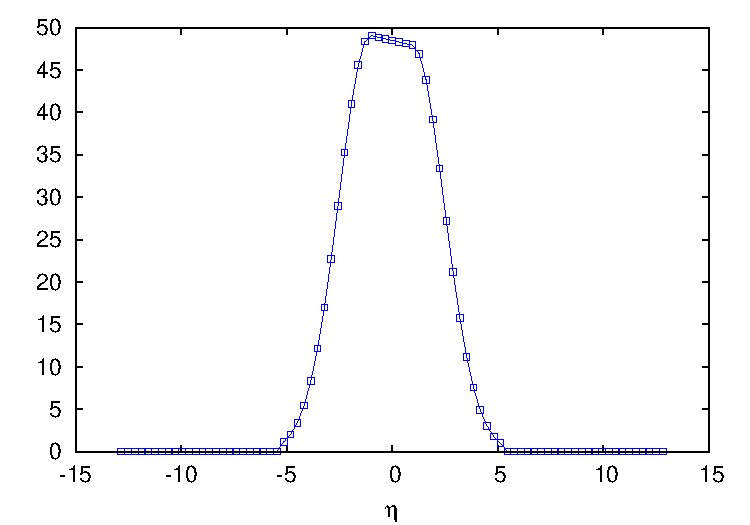
\includegraphics[width=8cm]{images/plot_en_vs_eta.pdf}
   \caption{Test F - Initial energy density vs $\eta$ at $\tau=1$ fm/c and $x=y=0$ (Glauber-MonteCarlo initialization).}
    \label{fig:endens-gmc3}
 \end{center}
\end{figure}
Now we plot the initial energy distribution on the $\eta=0$ (x,y) plane at $\tau=10.22$ fm/c (last output frame before the end of the simulation, i.e. when the maximum temperature on the grid was less than 137 MeV) (Fig. \ref{fig:endens-gmc94}).
\begin{lstlisting}[numbers=none, language=]
./fromecho2d.exe EPS0094.dat en_out94.dat x y
\end{lstlisting}
\begin{lstlisting}[numbers=none, language=]
gnuplot contour_out94.gp
\end{lstlisting}

\begin{figure}[!h]
 \begin{center}
  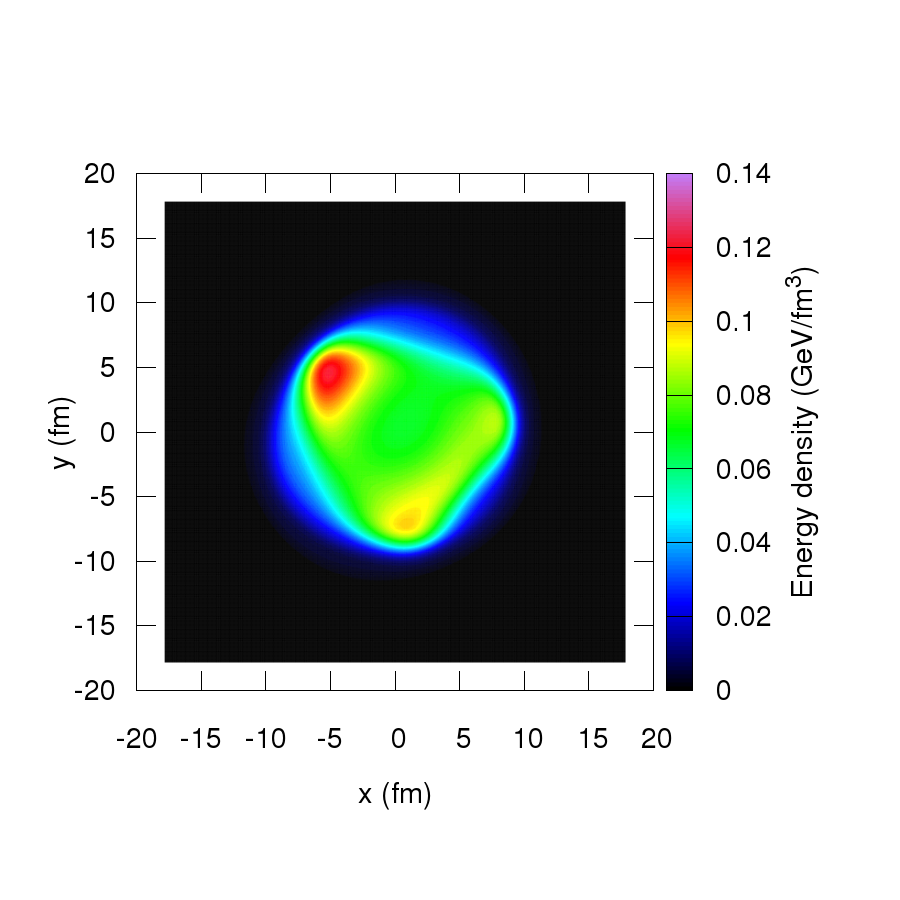
\includegraphics[width=8cm]{images/gmc_energy_density_contour_at_eta_0_tau10_22.png}
   \caption{Test F - Initial energy density distribution at $\tau=10.22$ fm/c with Glauber-MonteCarlo initialization.}
    \label{fig:endens-gmc94}
 \end{center}
\end{figure}

\section{Run with ``tilted'' initial conditions - test G}
In this example we run a simulation with Geometric Glauber initial conditions, without viscous effects, but with a ``tilted'' energy density distribution. The files related to this example can be found into the {\tt tests/testG} directory.\\
Using the same procedure shown in the previous example (test F), we draw a contour plot of the initial energy distribution, to visually verify the effect of ``tilting'' (Fig. \ref{fig:testG}).\\
\begin{figure}[!h]
 \begin{center}
  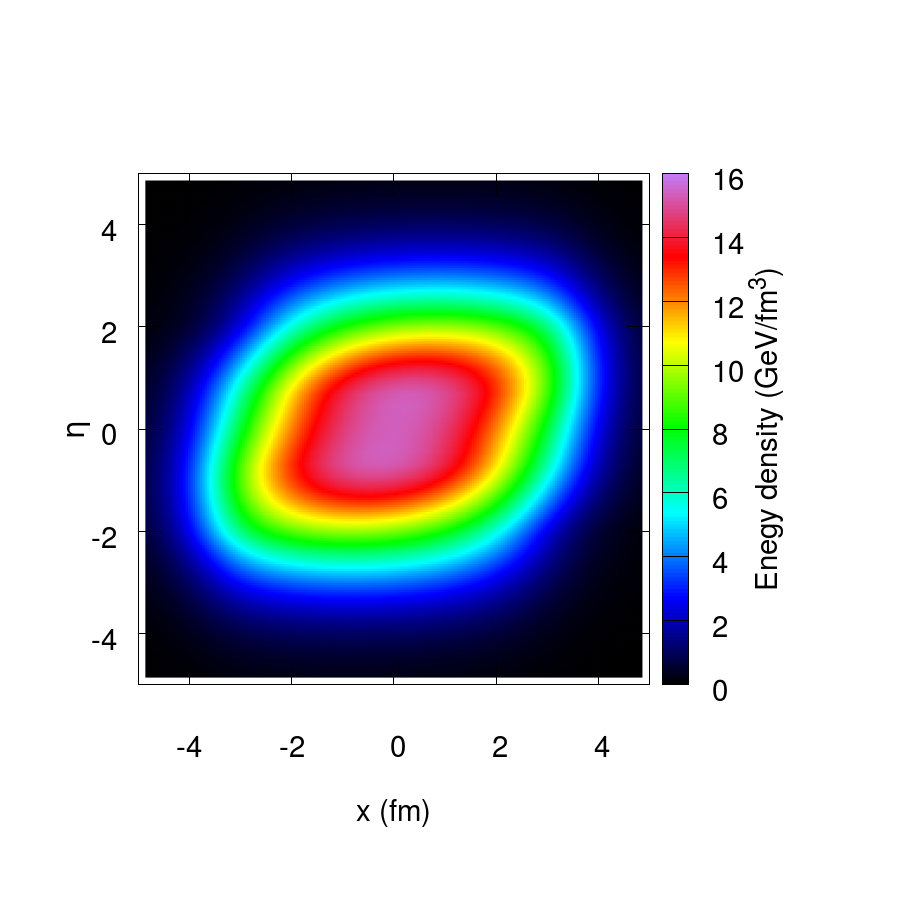
\includegraphics[width=8cm]{images/contour_energy_density_tau_1.png}
   \caption{Test G - Initial energy density distribution at $\tau=1$ fm/c.}
    \label{fig:testG}
 \end{center}
\end{figure}
Now, since this is a simulation without viscosity effects, we use the GDL postprocessing utilities to verify the conservation of total energy and angular momentum during the fluid evolution.\\
So, after copying from the tools directory into the {\tt outr0001} directory the {\tt readvar.pro} and {\tt ce.pro} scripts, we launch \emph{gdl} and we run them:
\begin{lstlisting}[numbers=none, language=]
GDL> readvar, 0001
\end{lstlisting}
\begin{lstlisting}[numbers=none, language=]
GDL> ce
\end{lstlisting}
getting, for $tau=1$ fm/c:
\begin{verbatim}
Total energy:        12400.207
J^y:       -5838.3068
\end{verbatim}
then, to see what are the total energy and the angular momentum $J^y$ at $\tau=11$ fm/c:
\begin{lstlisting}[numbers=none, language=]
readvar, 0101
\end{lstlisting}
\begin{lstlisting}[numbers=none, language=]
ce
\end{lstlisting}
getting:
\begin{verbatim}
Total energy:        12371.264
J^y:       -5834.8883
\end{verbatim}
So, in this run, total energy was conserved within a $\sim 0.2\%$ while , for $J^y$, within a $\sim 0.06\%$.\\


\chapter{Particle spectra production}\label{spectrachap}
We always refer to the Minkowski and Bjorken metrics 
respectively as
   \begin{align}
    &g_{M}^{\mu\nu}=\left( \begin{array}{cccc}
                        1&&&\\
                        &-1&&\\
                        &&-1&\\
                        &&&-1\\
                       \end{array}\right)&&
    &g^{\mu\nu}=\left( \begin{array}{cccc}
                        1&&&\\
                        &-1&&\\
                        &&-1&\\
                        &&&-\frac{1}{\tau^2}\\
                       \end{array}\right)&&
   \end{align}

We convert the description from hydro to particles, using the Cooper-Frye 
prescription.
Referring directly to the article by Cooper and Frye \cite{Cooper1974}:
\begin{align}
 E\dfrac{\de^3N_i}{\de p^3}=\dfrac{d^3N_i}{d	\mathrm{y} p_Tdp_Td\phi}=
\dfrac{g_i}{{(2\pi)}^3}\int_\Sigma{ \dfrac{p^\mu d^3\Sigma_\mu}
{\exp{\frac{u^\mu p_\mu-\mu_i}{T_{\mathrm{FO}}}}\pm 1}}
\label{eq:cooperfrye}
\end{align}
The index $i$ refers to the nature of the particle. Note that this time the 
rapidity $\mathrm{y}$ refers to the produced particle, and not the fluid! 
The decomposition of the particle four-momentum must be consistent with the 
Milne coordinates:
\begin{align}
p^\mu= \left(\begin{array}[c]{c}
\mt \cosh(\rap-\eta_s) 	\\
\pt \cos\phi			\\
\pt \sin\phi			\\
\frac{\mt}{\tau}\sinh(\rap-\eta_s)
\end{array}\right) \qquad 
\begin{array}[c]{c}
\mt = \sqrt{m_i^2 + \pt^2}\\
\pt= \sqrt{p_x^2 + p_y^2}\\
\rap= \frac{1}{2} \ln\left(\dfrac{E+p_z}{E-p_z}\right)
\end{array}
\label{eq:momentum}
\end{align}
The current version of the particle spectra production routines \textbf{only works in Milne (Bjorken) coordinates}.

\section{{\tt hypersuface.f90} in ECHO-QGP} \label{sec:hysu}
The task of the routine {\tt hypersuface.f90} included in ECHO-QGP is to find, 
store and print the coordinates of the hypersurface detected during the
hydrodinamic evolution. The user can choose the hypersuface to be isothermal or constant energy, using the switch HYP\_COMPU in the {\tt param.dat} file.

% % 
% % \hspace*{-1.2cm}
% % \fbox{ \tt \small
% %   \parbox{1.15\textwidth}{
% %  ! section for freezout hypersurface computation \\
% %  
% %   \begin{minipage}{0.2\textwidth} 
% %   HYP\_COMPU=1    \\ 
% %   FREEZKIND=0\\
% %   FREEZEVAL=0.13\\
% %   HYPSURFTI=0.1
% % \end{minipage}
% % \hspace*{0.05\textwidth}
% % \begin{minipage}{\textwidth}
% %  !0 disable / 1 enable hypersurface computation\\
% %  !0 freezout based on temperature - 1 freezeout based on energy density\\
% %  !freezeout threshold: temperature (GeV) or energy density (GeV/fm3)\\
% %  !time interval between hypersurfaces computations
% %  \end{minipage}
% % }}
% % \begin{description}
% %  \item[HYP\_COMPU] \textit{integer} It is a switch that enables or disables
% % the whole routine. It can only be 0 (OFF) or 1 (ON). If 0 it saves
% % computational time but it does not perform any decoupling technique.
% %  \item[FREEZKIND] \textit{integer} It allows to choose to perform the
% % decoupling finding a isothermal hypersuface (if set to 0) or a constant energy
% % density hypersuface (if set to 1). In both cases the value taken into account
% % as temperature or  energy density is listed below as FRREZEVAL.
% %  \item[FREEZEVAL] \textit{real} Numerical value of the temperature (GeV) or
% % energy density (\si{GeV/fm^3}) used to pinpoint the hypersurface.
% %  \item[HYPSURFTI]  \textit{real} Time interval (in fm )of the grid passed to the
% % hypersurface-finding routine. Sometimes to treat shocks it is useful to
% % set a very dense grid, but in order to compute the hypersurface a lesser dense
% % grid is needed, so it would be a waste of computing time to perform the check
% % at every hydro step.  
% % \end{description}

The routine checks in every space-time direction if two adjacent cells are one
above and one below the criterion. Let US refer to the cells with the index $i$,
being the direction positive with crescent $i$ (es. $x_{i+1}> x_i$
); and $F_\mathrm{i},F_\mathrm{i+1},F^*$ respectively the selected field
(temperature or energy density) in the adjacent cells and of the constant
hypersuface. Then we know that the hypersuface lies between the considered
cells if 
$$
(F_{i+1}-F^*)(F^*-F_{i})\geq0
$$
When this happens we store all the needed information, namely\\

\begin{minipage}[t]{0.45\textwidth}
\textbf{in the ideal case}\\
an array with 13 entries:\\
\begin{enumerate}
 \item $\tau$ or $t$
 \item $x$ 
 \item $y$ 
 \item $\eta$ or $z$
 \item $\rho$
 \item $v^x$
 \item $v^y$
 \item $v^\eta$ or $v^z$
 \item p
 \item dV$^{\perp \tau}$ or  dV$^{\perp t}$
 \item dV$^{\perp x}$
 \item dV$^{\perp y}$
 \item dV$^{\perp \eta}$ or  dV$^{\perp z}$
\end{enumerate}
\end{minipage}\:
\begin{minipage}[t]{0.45\textwidth}
\textbf{in the viscous case}\\
In addition to the ideal case, another array with 12 entries
\begin{enumerate}\setcounter{enumi}{13}
\item bulk
\item $\pi^{xy}$
\item $\pi^{xz}$ or  $\pi^{x\eta}$
\item $\pi^{yz}$ or  $\pi^{y\eta}$
\item $\pi^{xx}$
\item $\pi^{yy}$
\item $\pi^{zz}$ or  $\pi^{\eta \eta}$
\item $\pi^{tt}$ or  $\pi^{\tau \tau}$
\item $\pi^{tx}$ or  $\pi^{\tau x}$
\item $\pi^{ty}$ or  $\pi^{\tau y}$
\item $\pi^{tz}$ or  $\pi^{\tau \eta}$
\item $(e+p)T^2$  
\end{enumerate}
\end{minipage}\\


the variables are computed interpolating linearly, using a weight $w$:
$$w=\dfrac{F_i-F^*}{F_i-F_{i+1}}$$
The volume element in the bjorken case is defined as
\[
\de V=\left\lbrace
\begin{array}{cc}
\de V^{\perp \tau}= s^\tau \tau \Delta x \Delta y \Delta \eta &(\si{fm^3})\\
\de V^{\perp x}= s^x \tau \Delta \tau \Delta y \Delta \eta &(\si{fm^3})\\
\de V^{\perp y}= s^y \tau \Delta \tau \Delta x \Delta \eta &(\si{fm^3})\\
\de V^{\perp \eta}= \frac{s^\eta}{\tau} \Delta \tau \Delta x \Delta y 
&(\si{fm^2})\\
\end{array}\right.\qquad\mbox{with}\qquad
s^\mu=-sign\left(\dfrac{\partial T}{\partial x^\mu}\right)
\]
note that currently for most cells just one of the $\de V$ component is not
vanishing. \\


The above described array is printed in the file {\tt hypersuface.txt} in the 
output folder. This file contains as a first row the selected switch (namely 
{\tt FREEZKIND }), the temperature (in GeV) of the hypersuface and its energy 
density (\si{GeVfm^{-3}}). 
After the first row it contains a block for each time-step. The block head is an 
integer: it is the number of frozen cells contained which corresponds to the 
amount of lines to be read before finding another block. Each one of these lines 
is a frozen cell, where the column index refers to the array ``hypersurface''
described above. For the ideal case the columns are 13, for the viscous one the 
columns are 25.





\section{Particle spectra routines}
All the spectra routines are contained in the folder {\tt analisi}.
There are four separate programs: 
\begin{description}
 \item[thermal] which can be build with the command {\tt make thermal}
 \item[utils\_therm]  which can be build with the command {\tt make} {\tt utils\_them}
 \item[MCgen]  which can be build with the command {\tt make MCgen}
 \item[utils\_histogram]  which can be build with the command {\tt make}  {\tt utils\_histogram}
\end{description}
Issuing just the {\tt make} command, just {\tt thermal} and {\tt MCgen} are produced.

{\tt thermal} produces the averaged spectra of the selected particle specie, whereas {\tt MCgen} produces a ramdom sample of such particles. This last program needs some of the output files of the former, but since the computational load for {\tt thermal} is heavy, the user can exploit {\tt utils\_therm} to produce just the files needed by the Monte Carlo generator, saving time. {\tt utils\_histogram}, instead allows the user to re-arrange in different binnings the histogram produced by {\tt MCgen}


All these programs need the file {\tt settings.txt} to be carefully filled in. 
\section{How to configure the particle production}
 All the programs contained in the folder analisi
use as configuration file {\tt settings.txt}, although not all parameters are effectively used in each program. In the listing \ref{listing_settings} an example of the configuration file is provided.
As we did in 
ECHO-QGP configuration file, also this {\tt settings.txt} is divided into sections and most important needs \textbf{its structure not to be altered}.
\lstinputlisting[caption=Example of settings.txt, label=listing_settings, style=customtxt]{./images/settings.txt}

Despite all programs read the settings file, 
not all the variables are being used in each.
\subsection{ECHO-QGP related parameters}
This section contains the parametrs and the flags related to the hydrodynamic part of the simulation, such as the 
\begin{description}
\item[dim] \integer - flag. Sets the dimensionality of the ECHO-QGP simulation. Allowed  values are 2 or 3, for (1+2)-D and (3+1)-D simulations respectively.
 If the cross-check with the output with ECHO-QGP gives a different 
 dimensionality the code quits with en error message.
\item[visco\_hyd]  \integer - flag. Passes to the program the information about the ECHO-QGP simulation: must be 1 if the simulation was a viscous one, 0 if it was ideal. Note that the file containing the hypersurface information and the array listed in section \ref{sec:hysu} are allocated accordingly.
\item[visco\_spe]  \integer - flag. 
Enables(1) or disables(0) the viscous contributions to the distribution function in the spectra computation. It can only be activated when {\tt visco\_hyd=1}
\item[vorticity]  \integer - flag. 
Enables(1) or disables(0) the computation of thermal vorticity over the decoupling hypersurface. It needs the file \textit{hypersurf\_deriv.txt} produced by ECHO-QGP in the same directory containing  \textit{hypersurface.txt}
\item[nout] \integer - flag. 
It is the number of time-steps to be taken into 
account. If set to 0 the program reads all the time steps produced by ECHO-QGP, if not the program asks the user if the number of output is correct and wants a Y/N answer from the keyboard, followed by the return command to continue. This variable is very useful for debugging.
\end{description}

\subsection{Particle related parameters}
This section contains the parametrs related to the produced particles, such as the species and the momentum.\\


The programs in this section use concatenated loops over the momentum components, 
where we refer to the momentum components referring to equations  \ref{eq:momentum}, and using 
the transverse momentum $\pt$, the polar angle $\phi$ and the particle rapidity $\rap$ as the indipendent variables.
% in the program {\tt thermal.exe} we 
% compute the thermal spectra (see subsection \ref{sec:thermal}) 
% using three 
The three-dimensional grid in momentum is  thus
composed by {\tt npt}$\times${\tt nphi}$\times${\tt nrap} 
($N_{\pt} \times N_\phi \times N_\rap$). The points in each 
one of the three components are computed following the simple scheme\\

\begin{minipage}{0.4\textwidth}
 \begin{lstlisting}
dpt=(ptmax-ptmin)/npt
do i=1, npt
  pt(i)=ptmin+(i-0.5)*dpt
end do
\end{lstlisting}
\end{minipage}
\hspace{0.05\textwidth}
\begin{minipage}{0.4\textwidth}
 \begin{lstlisting}
dphi=(phimax-phimin)/nphi
do i=1, nphi
  phi(i)=phimin+(i-1.0)*dphi 
  ! we would like start with 0
end do
\end{lstlisting}
\end{minipage}\\
The particle rapidity initialization is very similar to the ones listed above, 
except the fact that the code checks whether the range is symmetric and tries 
to adjust $N_\rap$ (adding a point) to have the value 0 too.



% \[
% p^\mu = \left(\mt \cosh(\rap - \eta_s), \pt \cos\phi, \pt\sin\phi,
% \frac{\mt}{\tau}\sinh(\rap-\eta_s)\right)=(\si{fm^{-1}}, \si{fm^{-1}},
% \si{fm^{-1}}, \si{fm^{-2}} )
% \]
% NB {\color{red}  in the code there is no minus sign! the $s^\mu$ is
% already calculated to give all + signs}
% \begin{align*}
%  & p^\mu \de \Sigma_\mu = p^\mu \de \Sigma^\nu g_{\mu\nu}=\\
%  &\mt \cosh(\rap -\eta_s) \dVtau
%  -\pt \cos\phi \dVx 
%  -\pt \sin \phi \dVy
%  - \tau^2 \dfrac{\mt}{\tau} \sinh(\rap -\eta_s) \dVeta\\
%  &=\si{fm^2} 
% \end{align*}

\begin{description}
 \item[npt] \integer - value. Number of transverse momentum ($\pt$) points
\item[ptmin] \real - value. Minimum of the range in transverse momentum (${\pt}_{\rm min}$; GeV) 
\item[ptmax] \real - value. Maximum of the range in transverse momentum (${\pt}_{\rm max}$; GeV) 
\item[nphi]  \integer - value. Number of polar angle ($\phi$)  points
\item[phimin] \real - value. Minimum of the range in polar angle  ($\phi_{\rm min}$)
\item[phimax] \real - value. Maximum of the range in polar angle  ($\phi_{\rm max}$)
\item[nrap] \integer - value. Number of rapidity ($\rap$) points 
\item[rapmin] \real - value. Minimum of the range in rapidity ($\rap_{\rm min}$)
\item[rapmax] \real - value. Maximum of the range in rapidity ($\rap_{\rm max}$)
\item[listorseq] \integer - flag. It is the switch that allows the user to 
 change the set of particles to be used. 
 All the programs can use three different sets of particles. \\
In the folder {\tt eos\_data } must be present the file {\tt pdglist.txt}, which lists all the 
particle which can be included in the computation (one can see a human-readable 
table in the Appendix \ref{sec:particlelisting}). The code uses such table to 
read the particles features. The first integer number is the ID number of the 
particle, which we use in the settings file to identify it. 
 \textbf{listorseq}   can assume following values:
 \begin{enumerate} \setcounter{enumi}{-1}
  \item Uses ALL the particle listed in the file {\tt pdglist.txt}
  \item Uses a the particles included in the list, between the ID corresponding
  to ID\_START and the ID corresponding to ID\_STOP 
  \item Uses a list of particles, which IDs \underline{must be listed in the settings file, just after the {\tt part\_list} line}
 \end{enumerate}
 For the sake of clearness, we show in this section three examples of the using 
 of these options in the subsection \ref{sec:examples}
 \item[ID\_start] \integer - particle ID. Only used if {\tt listorseq=1}, 
 is the first particle in the  range the user wants to used
 \item[ID\_stop] \integer - particle ID. Only used if {\tt listorseq=1}, 
 is the last particle in the  range the user wants to used
  \item[part\_list]  \integer - value.   Only used if {\tt listorseq=2}, is the total
  number of particles listed in the settings file, \underline{which must correspond to the lines with the IDs after this parameter}.
  \item[antibar] \integer - flag. Since in the {\tt pdglist.txt} file there is no
  antibaryon listed, this switch enables (1) or disables (0) the production of the
  antibaryons corresponding to the listed baryons.
  \item[chempot] \integer - flag. If set to 0 it forces the chemical potentials 
  of all considered particles to be 0. If set to 1, the program reads the 
  chemical potential corresponding to the the given temperature from the file 
  {\tt chemical\_potential.txt} contained in the {\tt eos\_data} folder.
  \end{description}
  
  \section{Input-Ouput}
 The section of the file {\tt settings.txt} dedicated to the input/output 
 addresses simply contains  paths and  names:
  \begin{description}
  \item[inputdir] \chara *64 - path.  Path of the folder containing the 
  file {\tt hypersurface.txt}
  \item[ioutdir] \chara *64 - path. Path in which all the files produced by {\tt thermal} (and by {\tt utils\_therm}) are stored. The same path also contains the info used by {\tt MCgen}. 
  If the folder exists already, the content is replaced, while if the folder does not exist, a new one is created. 
  \item[mcoutdir] \chara *64 - path.    Path in which all the files produced by {\tt MCgen}  (and by {\tt utils\_histogram})   are stored. 
  If the folder exists already, the content is replaced, while if the folder does not exist, a new one is created. 
\end{description}

\section{Parameters for the Monte Carlo production}
In this section the user can find all the parameters for the Monte Carlo generation of particles. 
  \begin{description}
  \item[seed] \integer - flag and value. If 0 is given, the seed is automatically 
  generated and stored in the file \textit{report\_MCgen.txt} (placed in the folder specified by the path \textbf{mcoutdir})
  \item[ptbox] \real - value. Upper limit for the random sampling (from a uniform distribution) of the transverse momentum ($\pt$, GeV).
  \item[phibox] \real - flag and value. Upper limit for the random sampling (from a uniform distribution) of the polar angle ($\phi$). If set to 0 the upper limit is automatically set to $2\pi$
  \item[ybox] \real - value. Upper limit for the random sampling (from a uniform distribution) of the rapidity ($\rap$). 
  \end{description}
The user must be careful in the choice of {\tt ptbox},  {\tt phibox} and {\tt ybox}: given three random numbers $r_1, r_2, r_3 \in [0;1]$ the momentum is sampled with the formula:
\begin{align}
\pt &=  r_1\cdot {\tt ptbox}\\
\phi &= r_2\cdot {\tt phibox}\\
\rap &=  r_3\cdot 2\cdot {\tt ybox} -{\tt ybox}
\end{align}
so a bad choice of the upper limits can lead either to a wrong sampling ensable or a bottleneck in the code.
\begin{description}
  \item[oversmpl] \real - flag and value. This parameter allows the user to perform an oversampled (if the parameter is greater than 1) simulation, as well as an undersampled (if the parameter is less than 1) simulation. The histograms computation automatically takes care of this parameter renormalizing them. This parameter is mainly useful during the debugging stage.   
\end{description}

\subsubsection{Histogram related parameters}\label{sec:histogram}
When the Monte Carlo production of the particles is terminated, some histograms are automatically calculated, in order to be compared with the averaged spectra.
Such histograms calculation can also be performed independently with the program {\tt utils\_histogram}. This section specifies the binning of such histograms.
\begin{description}
 \item[mxv\_pt]  \real - value. Maximum value in the transverse momentum histogram
 \item[mnv\_pt]  \real - value. Minimum value in the transverse momentum histogram
 \item[mxv\_ang] \real - value. Maximum value in the polar angle histogram
 \item[mnv\_ang] \real - value. Minimum value in the polar angle histogram
 \item[mxv\_y]   \real - value. Maximum value in the   particle rapidity histogram 
 \item[mnv\_y]   \real - value. Minimum value in the particle rapidity histogram 
 \item[binpt]  \integer - value.   Number of bins in the   transverse momentum histogram
 \item[binphi] \integer - value.   Number of bins in the polar angle       histogram
 \item[binrap] \integer - value.   Number of bins in the particle rapidity    histogram
\end{description}


\section{Examples of particles subset:}\label{sec:examples}
The IDs of the particles are listed into the file {\tt eos\_data/pdglist.txt}.

% % ---
\subsection{Producing all available particles: {\tt listorseq=0}}
We provide here an example of the particle section in the setup file, 
for a simulation including \textit{\textbf{ALL the particles}}, comprehensive of antibaryons.
We also set as active in the computation, the appropriate and the chemical potential in {\tt settings.txt}\\
Please note in \ref{listing_settings_all} that there is NO line after the {\tt part\_list} line, and the 
variable {\tt part\_list} itself is set to 0.\\
\lstinputlisting[firstline=8, lastline=23, caption=Example of the section in settings.txt producing all the available particles., label=listing_settings_all, style=customtxt]{./images/settings_all.txt}

% % ---
\subsection{Producing an interval of listed particles: {\tt listorseq=1}}

Let's assume that the user wants to produce all the particle listed in \textit{pdglist.txt} \textbf{between two given IDs}, say $\pi^+$ (with ID 211) and $\eta$ (with ID 221), 
which are: $\pi^+, \pi^0, \pi^-, K^+, K^-, K^0, \overline{K^0}, \eta$.
The fastest way to configure \textit{settings.txt} is to set {\tt listorseq=1}, 
{\tt ID\_start=211} and {\tt ID\_stop=221}.
Here we provide an example setup for a simulation producing such ensemble, without the production of antibaryons, and with the appropriate chemical potential.
Please note that still there is NO line after the {\tt part\_list} line, and the 
variable {\tt part\_list} itself is set to 0.\\
\lstinputlisting[firstline=8, lastline=23, caption=Example of  the section in  settings.txt producing a custom sequence of particles., label=listing_settings_seq, style=customtxt]{./images/settings_seq.txt}


% % ---
\subsection{Producing a detailed list of particles {\tt listorseq=2}}
Within this configuration, the user can pick any list of particles to produce, and specify their ID in any order. Let's assume that the user wants to produce 
$\pi^+$ (ID 211), 
$K^-$ (ID -321), 
$\rho^0$ (ID 113), 
$\omega$ (ID 223)
 $p$ (ID 2212) and $\bar{p}$ (not listed); for a total amount of 5 
 listed particle and 1 anti-baryon.
In the \textit{settings.txt} file the variable {\tt part\_list} must contain the numeber of listed particles ({\tt part\_list=5}) and the IDs of the particles must be placed one-per-line just after this parameter (as shown in the listings \ref{listing_settings_list}).

\lstinputlisting[firstline=8, lastline=28, caption=Example of the section in settings.txt producing a custom list of particles., label=listing_settings_list, style=customtxt]{./images/settings_list.txt}



% %  ---
\subsection{Producing the standard subset of particles{\tt listorseq=3}}
Example setup for a simulation including the standard subset of particles:
$\pi^+,\pi^0,\pi^-,K^+,K^0,\bar{K^0},K^-,\eta,\omega, p, n, \Lambda, \Sigma^+, \Sigma^0, \Sigma^-, \Xi^0, \Xi^-$.\\
Please note that still there is NO line after the {\tt part\_list} line, and the 
variable {\tt part\_list} itself is set to 0.\\
\lstinputlisting[firstline=8, lastline=23, caption=Example of settings.txt producing the standard subset of particles., label=listing_settings_stable, style=customtxt]{./images/settings_stable.txt}


\addcontentsline{toc}{chapter}{References}
\bibliographystyle{ieeetr}
\bibliography{bibliography}

\end{document}
